% \documentclass[reprint, amsmath,amssymb,aps,pra]{revtex4-2}
\documentclass[11pt,reqno]{amsart}

\usepackage[pdfborder={0 0 0.5 [3 2]}, plainpages=false]{hyperref}%
\usepackage[left=1in,right=1in,top=1in,bottom=1in]{geometry}%
% \usepackage[shortalphabetic]{amsrefs}%
\usepackage{amsmath}
\usepackage{enumerate}
% \usepackage{enumitem}
\usepackage{amssymb}                
\usepackage{amsmath}                
\usepackage{amsfonts}
\usepackage{amsthm}
\usepackage{bbm}
\usepackage[table,xcdraw]{xcolor}
% \usepackage{float}
\usepackage{booktabs}
\usepackage{svg}
\usepackage{mathtools}
\usepackage{cool}
\usepackage{url}
\usepackage{graphicx,epsfig}
\usepackage{makecell}
\usepackage{array}

\usepackage{subcaption}
\captionsetup{font={small},skip=0.25\baselineskip}
\captionsetup{justification=raggedright}
\captionsetup[subfigure]{font={small}, skip=1pt, singlelinecheck=false}

\usepackage[capitalize,nameinlink]{cleveref}
% Per SIAM Style Manual, "section" should be lowercase
\crefname{section}{section}{sections}
\crefname{subsection}{subsection}{subsections}
\Crefname{section}{Section}{Sections}
\Crefname{subsection}{Subsection}{Subsections}

% Per SIAM Style Manual, "Figure" should be spelled out in references
\Crefname{figure}{Figure}{Figures}

% Per SIAM Style Manual, don't say equation in front on an equation.
\crefformat{equation}{\textup{#2(#1)#3}}
\crefrangeformat{equation}{\textup{#3(#1)#4--#5(#2)#6}}
\crefmultiformat{equation}{\textup{#2(#1)#3}}{ and \textup{#2(#1)#3}}
{, \textup{#2(#1)#3}}{, and \textup{#2(#1)#3}}
\crefrangemultiformat{equation}{\textup{#3(#1)#4--#5(#2)#6}}%
{ and \textup{#3(#1)#4--#5(#2)#6}}{, \textup{#3(#1)#4--#5(#2)#6}}{, and \textup{#3(#1)#4--#5(#2)#6}}

% But spell it out at the beginning of a sentence.
\Crefformat{equation}{#2Equation~\textup{(#1)}#3}
\Crefrangeformat{equation}{Equations~\textup{#3(#1)#4--#5(#2)#6}}
\Crefmultiformat{equation}{Equations~\textup{#2(#1)#3}}{ and \textup{#2(#1)#3}}
{, \textup{#2(#1)#3}}{, and \textup{#2(#1)#3}}
\Crefrangemultiformat{equation}{Equations~\textup{#3(#1)#4--#5(#2)#6}}%
{ and \textup{#3(#1)#4--#5(#2)#6}}{, \textup{#3(#1)#4--#5(#2)#6}}{, and \textup{#3(#1)#4--#5(#2)#6}}

% Make number non-italic in any environment.
\crefdefaultlabelformat{#2\textup{#1}#3}

\def\noi{\noindent}
\def\T{{\mathbb T}}
\def\R{{\mathbb R}}
\def\N{{\mathbb N}}
\def\C{{\mathbb C}}
\def\Z{{\mathbb Z}}
\def\P{{\mathbb P}}
\def\E{{\mathbb E}}
\def\Q{\mathbb{Q}}
\def\ind{{\mathbb I}}
\def\calI{{\mathcal I}}
\def\calL{{\mathcal L}}
\def\calH{{\mathcal H}}
\def\Lw{{\mathcal{L}_\omega}}

\DeclareMathOperator{\spn}{span}
\DeclareMathOperator{\ran}{range}
\DeclareMathOperator{\diag}{diag}
\DeclareMathOperator{\md}{mod}
\DeclareMathOperator{\RR}{Re}
\DeclareMathOperator{\II}{Im}

\newtheorem{lemma}{Lemma}
\newtheorem{theorem}{Theorem}
\newtheorem{corollary}{Corollary}
\newtheorem{definition}{Definition}
\newtheorem{proposition}{Proposition}
\newtheorem{hypothesis}{Hypothesis}

\graphicspath{ {images/} }

\begin{document}

\title{Spatiotemporal dynamics of a twisted, circular waveguide array}

\author{Ross Parker}
\address{Department of Mathematics, Southern Methodist University, 
Dallas, TX 75275, USA}
\email{rhparker@smu.edu}

\author{Yannan Shen} 
\address{Department of Mathematics, University of Kansas, Lawrence, KS 66045, USA}
\email{yshen@ku.edu}

\author{Alejandro Aceves}
\address{Department of Mathematics, Southern Methodist University, 
Dallas, TX 75275, USA}
\email{aaceves@smu.edu}

\author{John Zweck}
\address{Department of Mathematics, The University of Texas at Dallas, 
Richardson, TX 75080, USA}
\email{zweck@utdallas.edu}

\begin{abstract}
    We consider stuff.
\end{abstract}

\maketitle

\section{Introduction}

Multi-core optical fibers, optical waveguides which contain multiple fiber  cores within a single cladding, have important applications in optical communications, as well as diverse fields such as biomedical imaging and experimental physics \cite{Ortiz2018}. Addition of a twist to a circular multi-core fiber allows for fine control of diffraction and light transfer, in a similar manner to axis bending in linear waveguide arrays \cite{Longhi2005}. Initial mathematical work on light propagation in twisted, circular, multi-core fibers with was done in \cite{Longhi2007,Longhi2007b,Garanovich2012}, in which coupled mode equations modeling optical transmission were derived. In non-dimensionalized form (and in the setting of no optical gain or loss) these are given by
\begin{equation}\label{eq:coupledmode}
i \partial_z c_n + k \left(e^{i\phi}c_{n-1} + e^{-i\phi}c_{n+1} \right) + |c_n|^2 c_n = 0,
\end{equation}
for $n = 1, \dots, N$, where $N$ is the number of fibers in the ring, and the indices $n$ are taken $\md n$ due to the circular geometry (\cref{fig:circle}). The complex amplitudes $c_n(z)$ represent the localized field amplitude in each waveguide, the independent variable $z$ is the axis of propagation, the parameter $k$ is the non-dimensional strength of the nearest-neighbor coupling of the waveguides in the ring, and $\phi = 4 \pi^2 \epsilon n_s R^2/N \lambda$ is the Peierls phase introduced by the twist \cite{Longhi2007,Peierls1933}, where $n_s$ the refractive index of the substrate, $R$ is the radius of the circular ring, and $\lambda$ is the wavelength of the propagating field \cite{castro2016}. We note that in this model, the intensity $c_n(z)$ of each waveguide is independent of the time $t$.

\begin{figure}
\begin{center}
\includegraphics[width=5cm]{circle}
\end{center}
\caption{Twisted, circular, multi-core fiber consisting of $N$ waveguides.}
\label{fig:circle}
\end{figure}

Twisted multi-core fibers have applications in distributive sensing, in which position, temperature, strain and acoustic signals can be detected along the entire length of the fiber \cite{Gannot2014,Westbrook2017}. Of particular note is shape sensing, in which the shape of the optical fiber can be reconstructed using measurements of light transmission and scattering through the fiber. The fiber twist permits the establishment of a topological state in the fiber, in which the intensity in one (or more) of the cores is completely suppressed. A six-core twisted optical fiber was considered in \cite{castro2016}, and asymptotic analysis showed that if the bulk of the optical intensity is confined to a single fiber in the ring, the opposite fiber in the ring is suppressed, to leading order, when $\phi = \pi/6$. This phenomenon is discussed as an optical analogue of Aharonov-Bohm (AB) suppression of tunneling in \cite{Ornigotti2007,Parto2017,Parto2019}; the fiber twist plays the role of the magnetic flux in the quantum mechanical system \cite{Loss1992}. This suppression effect was shown analytically for a four-core optical fiber when $\phi=\pi/4$ in \cite{Parto2019}. In \cite{parker2021}, we extended this analysis to standing waves, solutions of the form $c_n = a_n e^{i (\omega z + \theta_n) }$ which are constant in amplitude and oscillatory in $z$. We showed that when the number of fibers $N$ is even, standing wave solutions exist in which the bulk of the intensity is contained in a single fiber core, and the intensity in the opposite core in the ring is completely suppressed for all $z$ when $\phi = \pi/N$. Using numerical spectral computation and evolution experiments, we showed that these standing wave solutions are stable, and we also extended these results to the $N$ odd case.

In what follows, we extend these results to a model incorporating a second-order temporal dispersion term, as is found in the nonlinear Schr\"odinger equation
\begin{align}\label{eq:cnz}
&i\partial_z c_n + \partial_t^2 c_n + k\left(e^{i\phi}c_{n-1}+e^{-i\phi}c_{n+1}\right)+|c_n|^2 c_n = 0 && n = 1, \dots, N,
\end{align}
where the complex amplitudes $c_n$ are now functions of both $z$ and $t$. Using asymptotic analysis, we derive leading order expressions for solutions in which the bulk of the intensity is contained in a single core. We demonstrate that optical suppression also occurs in this model, to leading order, when the number of cores $N$ is even, and phase parameter $\phi$ is given by $\phi=\pi/N$. This paper is organized as follows. [SECTION SUMMARY].

% In \cref{sec:model}, we discuss the mathematical model we are using

\section{Mathematical model}\label{sec:model}

We start by discussing the mathematical model \cref{eq:cnz} we will be investigating. Let $c = (c_1, \dots, c_n)^T$. We can write \cref{eq:cnz} in matrix form as
\begin{align}\label{eq:cz}
i \partial_z c + \partial_t^2 c + k A(\phi) c + \diag\left(|c_n|^2\right)c = 0,
\end{align}
where $\diag\left(|c_n|^2\right)$ is the diagonal matrix with diagonal entries $\{|c_1|^2, \dots, |c_N|^2\}$, and $A(\phi)$ is the periodic, tri-diagonal, banded matrix
\begin{align}
A = \begin{pmatrix}
0 & e^{-i \phi} & & \dots & e^{i \phi} \\
e^{i \phi} & 0 & e^{-i \phi} & & & \\
& \ddots & \ddots & \ddots &  & \\
 & &e^{i \phi}  & 0 & e^{-i \phi}  \\
e^{-i \phi}& \dots & & e^{i \phi} & 0
\end{pmatrix}.
\end{align}
Equation \cref{eq:cnz} is Hamiltonian, with energy given by
\begin{align}\label{eq:Hc}
\calH(c) = \sum_{n=1}^N \int_{-\infty}^\infty 
\left(
|\dot{c}_n|^2 - \frac{1}{2}|c_n|^4 - e^{i\phi}( c_{n-1}c_n^* + c_{n+1}^* c_n) 
- e^{-i \phi}( c_{n-1}^*c_n + c_{n+1} c_n^*) \right) dt,
\end{align}
where the overdot denotes differentiation with respect to $t$, and the star denotes complex conjugation. We can write the system in standard Hamiltonian form by taking $q_n = \RR c_n$ and $p_n = \II c_n$, so that equation \cref{eq:cnz} becomes
\begin{equation}
\partial_z (q_1, \dots, q_N, p_1, \dots, p_N)^T
 = J \nabla H(q_1, \dots, q_N, p_1, \dots, p_N).
\end{equation}
$J$ is the standard symplectic matrix
\[
J = \begin{pmatrix}
0 & I_n \\ -I_n & 0
\end{pmatrix},
\]
with $I_n$ the $N \times N$ identity matrix, and the Hamiltonian \cref{eq:Hc} is written in terms of the $q_n$ and $p_n$ as
\begin{equation}\label{eq:Hqp}
\begin{aligned}
\calH(q_1, \dots, q_N, &p_1, \dots, p_N) = \sum_{n=1}^N \int_{-\infty}^\infty 
\Big(
\dot{q}_n^2 + \dot{p}_n^2 - \frac{1}{2}(q_n^2 + p_n^2)^2 \\
&- \left[(p_{n-1} + p_{n+1}) \cos\phi - (q_{n-1} - p_{n+1}) \sin \phi\right] p_n \\
&- \left[(p_{n-1} - p_{n+1}) \sin\phi + (q_{n-1} + p_{n+1}) \cos \phi\right] q_n
\Big) dt,
\end{aligned}
\end{equation}

\section{Standing waves}\label{sec:standing}

We are interested in finding standing wave solutions of the form $c_n(t) e^{i \omega z}$, which are oscillatory in $z$ with frequency $\omega$ and complex amplitude $c_n(t)$ depending only on $t$. Substituting this ansatz into \cref{eq:cnz}, a standing wave solution satisfies the system of $N$ coupled ordinary differential equations
\begin{align}\label{eq:standingwave}
\partial_t^2 c_n + k\left(e^{i\phi}c_{n-1}+e^{-i\phi}c_{n+1}\right)+|c_n|^2 c_n - \omega c_n = 0,
\end{align}
where the subscripts $n$ are taken $\md N$. Letting $c = (c_1, \dots, c_n)^T$, we can write this in matrix form as 
\begin{align}\label{eq:standingwavematrix}
\partial_t^2 c + k A(\phi) c + \diag\left(|c_n|^2 \right)c  - \omega c = 0
\end{align}
When the coupling parameter $k=0$, which is known as the anti-continuum (AC) limit, this reduces to $N$ independent copies of the standing wave equation for the NLS equation. The solution at each site is either 0 or the NLS soliton
\begin{equation}\label{eq:NLSsoliton}
\psi(t) = \sqrt{2 \omega} \sech(\sqrt{\omega} t).
\end{equation}
Due to the gauge symmetry of NLS, we can multiply \cref{eq:NLSsoliton} by $e^{i \theta}$ for any $\theta$. Next, we write $c_n(t)$ as
\begin{equation}\label{eq:cnansatz}
c_n(t) = a_n(t)e^{i \theta_n(t)},
\end{equation}
where we have separated each complex amplitude $c_n(t)$ into its real amplitude $a_n(t)$ and phase $\theta_n(t)$. Substituting this into \cref{eq:standingwave}, we obtain the equation
\begin{align*}
e^{i \theta_n}&\left[ (\ddot a_n - a_n (\dot \theta_n)^2) 
+ i ( a_n \ddot\theta_n + 2 \dot a_n \dot \theta_n ) \right] \\
&+ k\left(e^{i\phi}a_{n-1}e^{i \theta_{n-1}} +e^{-i\phi}a_{n+1}e^{i \theta_{n+1}}\right)+|a_n|^2 a_n e^{i \theta_n} - \omega a_n e^{i \theta_n} = 0.
\end{align*}
where we have suppressed the dependence on $t$ and used the overdot notation for derivatives with respect to $t$ for convenience. Dividing by $e^{i \theta_n}$, this becomes
\begin{equation}\label{eq:st2}
\begin{aligned}
(\ddot a_n &- a_n (\dot \theta_n)^2) 
+ i ( a_n \ddot\theta_n + 2 \dot a_n \dot \theta_n )\\
&+ k\left(a_{n-1}e^{-i[(\theta_n - \theta_{n-1}) - \phi]} + a_{n+1}e^{i[(\theta_{n+1} - \theta_{n}) - \phi]} \right)+a_n^3 - \omega a_n = 0,
\end{aligned}
\end{equation}  
which we can split up into real and imaginary parts to get
\begin{align}
&\ddot a_n - a_n (\dot \theta_n)^2 +
 k\left(a_{n-1}\cos[(\theta_n - \theta_{n-1}) - \phi] + a_{n+1}\cos[(\theta_{n+1} - \theta_{n}) - \phi] \right)+a_n^3 - \omega a_n = 0 \label{eq:st2real} \\
&a_n \ddot\theta_n + 2 \dot a_n \dot \theta_n
+ k\left(-a_{n-1}\sin[(\theta_n - \theta_{n-1}) - \phi] + a_{n+1}\sin [(\theta_{n+1} - \theta_{n}) - \phi] \right) = 0. \label{eq:st2imag}
\end{align}

\section{Asymptotic solutions}\label{sec:asymp}

We assume for now that the bulk of the intensity is contained a single node, which we will call the primary core and label $n=0$. We will take the number of waveguides $N$ to be even, although we will comment [IN A LATER SECTION] about what occurs when $N$ is odd. We will call the waveguide directly opposite the primary core the opposite core, which we label $n=N/2$. The remaining nodes in the ring are labeled $\pm n$, for $n = 1, \dots, N/2-1$, where we count clockwise around the ring for positive $n$ and counterclockwise for negative $n$. See \cref{fig:symm6} for the labeling scheme for $N=6$. Numerical parameter continuation experiments suggest that for $N$ even, there exist solutions with the following symmetries (see \cref{fig:symm6} for an illustration when $N=6$):
\begin{equation}\label{eq:symm}
\begin{aligned}
a_{-n}(t) &= a_{n}(t) && \qquad n = 1, \dots, N/2 \\
\theta_{-n}(t) &= -\theta_{n}(t) && \qquad n = 1, \dots, N/2 \\
\theta_0(t) &= 0 \\
\theta_{N/2}(t) &= 0.
\end{aligned}
\end{equation} 
We verify in \cref{app:symm} that these symmetry conditions are consistent, and we will look for a solution with these specific symmetries. 

\begin{figure}
\begin{center}
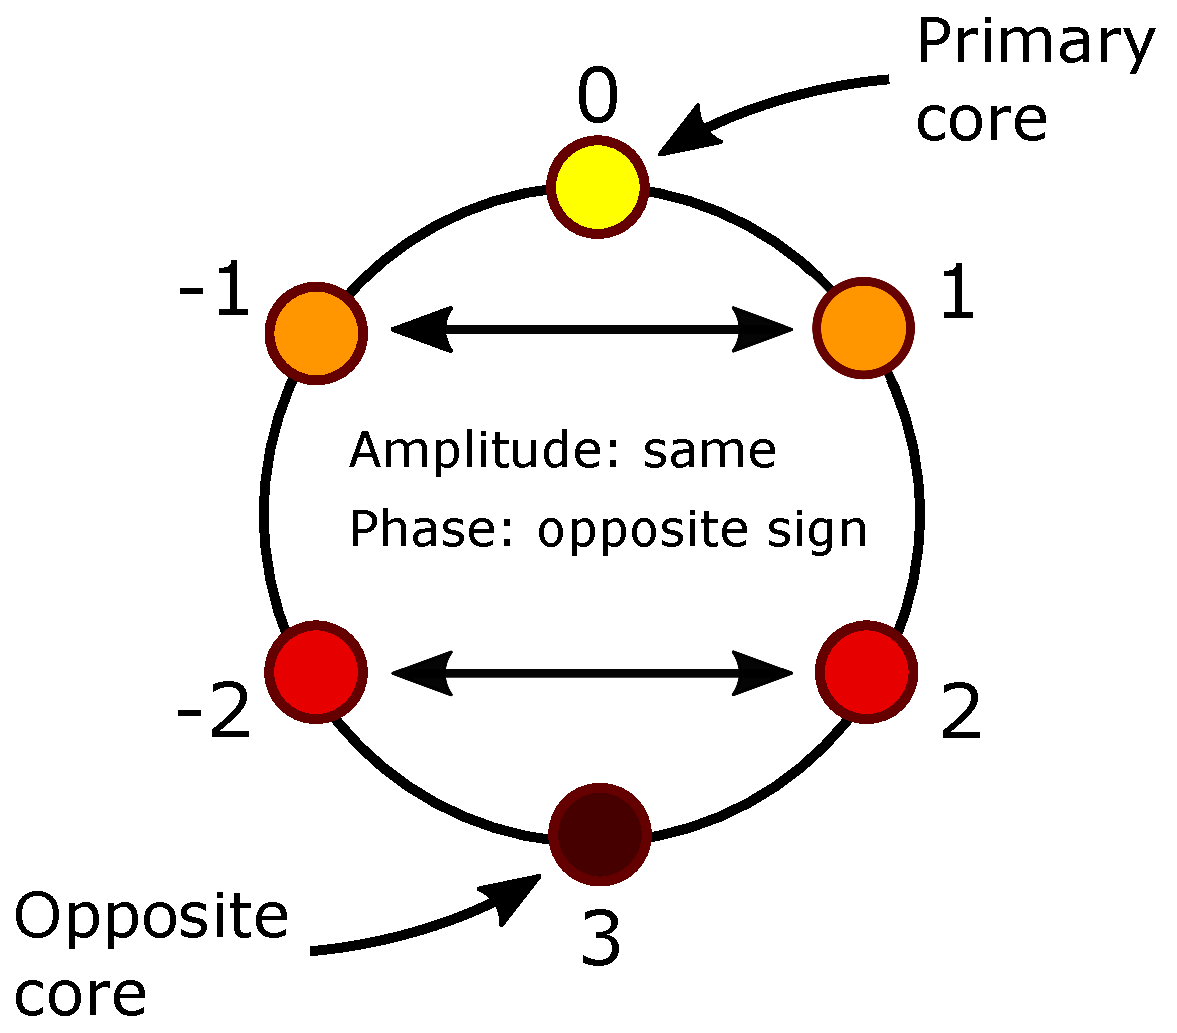
\includegraphics[width=7cm]{symm6}
\end{center}
\caption{Symmetry relations and site labeling in twisted, circular, multi-core fiber consisting of 6 waveguides.}
\label{fig:symm6}
\end{figure}

To find a leading order approximation for a solution to \cref{eq:st2}, we will assume that the amplitudes $a_n(t)$ and phases $\theta_n(t)$ have power series expansions in the coupling parameter $k$. Furthermore, we will assume that these terms have the following orders of magnitude in $k$, which are suggested by numerical parameter continuation experiments:
\begin{equation}\label{eq:basicseries}
\begin{aligned}
a_0(t) &= \psi(t) + \mathcal{O}\left(k\right) \\
a_n(t) &= \mathcal{O}\left(k^n\right) && n = 1, \dots, N/2 \\
\theta_n(t) &= n \phi + \mathcal{O}\left(k^{N - 2n}\right) && n = 1, \dots, N/2-1
\end{aligned}
\end{equation}
Since we wish node 0 to contain the bulk of the intensity, the leading order term for $a_1(t)$ is the NLS soliton $\psi(t)$, and the rest of the terms are of order $k$ or higher. The form of equation \cref{eq:st2} suggests that $a_n = \mathcal{O}(k a_{n_1})$, from which we obtain the ansatz for $a_n$ in \cref{eq:basicseries}. It follows from the ansatz for $\theta_n$ that, for $n = 1, \dots, N/2-1$, we have $\theta_n - \theta_{n-1} - \phi = \mathcal{O}\left(k^{N - 2n}\right)$. This implies that the cosine terms in \cref{eq:st2real} and the sine terms in \cref{eq:st2imag} are 1 and 0, respectively, to leading order.

Following the procedure detailed in \cref{app:asymp}, we obtain a solution to \cref{eq:st2} of the following form:
\begin{equation}\label{eq:asympsol}
\begin{aligned}
a_0(t) &= \psi(t) + k^2 \tilde{a}_0(t) + \mathcal{O}(k^3) \\
a_n(t) &= k^n \tilde{a}_n(t) + \mathcal{O}(k^{n+1}) && n = 1, \dots, N/2 \\
\theta_n(t) &= n \phi + k^{N - 2n} \tilde{\theta}_n(t) 
+ \mathcal{O}(k^{N - 2n+1}) && n = 1, \dots, N/2-1.
\end{aligned}
\end{equation}
For $n = 1, \dots, N/2$, $\tilde{a}_n(t)$ is defined recursively as 
\begin{equation}\label{eq:tildean}
\begin{aligned}
\tilde{a}_1(t) &= (\omega - \partial_t^2)^{-1} \psi(t) \\
\tilde{a}_n(t) &= (\omega - \partial_t^2)^{-1} \tilde{a}_{n-1}(t) && n = 2, \dots, N/2-1 \\
\tilde{a}_{N/2}(t) &= 2 \cos( N\phi/2)(\omega - \partial_t^2)^{-1} \tilde{a}_{N/2-1}(t),
\end{aligned}
\end{equation}
where each function $\tilde{a}_n(t)$ is defined in terms of the function $\tilde{a}_{n-1}(t)$, which is one closer to the primary core. The linear operator $(\omega - \partial_t^2)$ is invertible, as discussed in \cref{app:asymp}. We can write the equations \cref{eq:tildean} in terms of the NLS soliton $\psi(t)$ as
\begin{equation}\label{eq:tildeanpsi}
\begin{aligned}
\tilde{a}_n(t) &= (\omega - \partial_t^2)^{-n} \psi(t) && n = 1, \dots, N/2-1 \\
\tilde{a}_{N/2}(t) &= 2 \cos( N\phi/2)(\omega - \partial_t^2)^{-N/2} \psi(t).
\end{aligned}
\end{equation}
Note that $\tilde{a}_n(t)$ does not depend on $\phi$, except for when $n=N/2$. The remainder term $\tilde{a}_0(t)$ from node 0 can be found by solving the equation
\begin{equation}\label{eq:tildea0eq}
\left( \partial_t^2 - \omega + 3 \psi^2 \right) \tilde{a}_0(t) = -2 \tilde{a}_1(t) =
-2 (\omega - \partial_t^2)^{-1} \psi(t),
\end{equation}
with the condition that $\tilde{a}_0(t) \perp \dot \psi(t)$.

For the angles, we obtain the following recursive formulas for the products $\tilde{a}_n(t)\tilde{\theta}(t)$:
\begin{equation}\label{eq:tildeantn}
\begin{aligned}
\tilde{a}_{N/2-1}(t) \tilde{\theta}_{N/2-1}(t) &= -\sin(N \phi/2) (\omega - \partial_t^2)^{-1} \tilde{a}_{N/2}(t) \\
\tilde{a}_n(t) \tilde{\theta}_n(t) &= (\omega - \partial_t^2)^{-1} \left( \tilde{a}_{n+1}(t) \tilde{\theta}_{n+1}(t) \right) && n = 1, \dots, N/2-2,
\end{aligned}
\end{equation}
where each product $\tilde{a}_n(t) \tilde{\theta}_n(t)$ is defined in terms of the product $\tilde{a}_{n+1}(t) \tilde{\theta}_{n+1}(t)$, which is one further from the primary core. Note that these involve the terms $\tilde{a}_n(t)$, which were computed above. For $n = 1, \dots, N/2-2$, we can write the expression for $\tilde{a}_n(t) \tilde{\theta}_n(t)$ in terms of $\tilde{a}_{N/2-1} \tilde{\theta}_{N/2-1}$ as
\begin{align*}
\tilde{a}_n(t) \tilde{\theta}_n(t) &= (\omega - \partial_t^2)^{-(N/2-n-1)} \left( \tilde{a}_{N/2-1}(t) \tilde{\theta}_{N/2-1}(t) \right) && n = 1, \dots, N/2-2.
\end{align*}
Substituting \cref{eq:tildeanpsi} for $\tilde{a}_n(t)$ and simplifying, we can again write everything in terms of $\psi(t)$ to get
\begin{equation}\label{eq:tildeantnpsi}
\begin{aligned}
\tilde{a}_n(t) \tilde{\theta}_n(t) &= -\sin(N \phi) (\omega - \partial_t^2)^{-(N-n)} \psi(t) && n = 1, \dots, N/2-1.
\end{aligned}
\end{equation}
We can solve for $\tilde{\theta}_n(t)$ by dividing by $\tilde{a}_n(t)$, although we note that we have to be careful when doing this since $\tilde{a}_n(t) \rightarrow 0$ as $t \rightarrow \pm \infty$.

When $\phi = \pi/N$, it follows from \cref{eq:tildeanpsi} that $\tilde{a}_{N/2}(t) = 0$. Thus, as in the case without temporal dispersion, the intensity at the opposite site in the ring is suppressed at this value of the twist parameter $\phi$. It is important to note, however, that this choice of $\phi$ only zeros out the leading order term in the asymptotic expansion for $a_{N/2}(t)$, which is $\mathcal{O}(N/2)$. The intensity at the opposite site may not be completely suppressed due to the presence of higher order terms (of order $\mathcal{O}(k^{N/2+1})$ and higher) in the expansion for $a_{N/2}(t)$ that we have not computed. Similarly, it follows from \cref{eq:tildeantnpsi} that $\tilde{a}_n(t) \tilde{\theta}_n(t) = 0$ for all $n$ when $\phi = \pi/N$, which zeros out the leading order term in the expansions for $\theta_n(t)$ for all $n$. These findings are confirmed numerically in the next section.


\section{Numerical results}\label{sec:numerics}

First, we construct standing wave solutions to \cref{eq:standingwave} by using parameter continuation from the anti-continuum (AC) limit ($k=0$). To do this, we take $c_n = u_n + i v_n$ in \cref{eq:standingwave}, and separate real and imaginary parts to get
\begin{equation}\label{eq:standingwavesep}
\begin{aligned}
&\partial_t^2 u_n + k\left( (u_{n-1} + u_{n+1}) \cos \phi ) - (v_{n-1} - v_{n+1})\sin \phi \right) + (u_n^2+v_n^2) u_n - \omega u_n= 0, \\
&\partial_t^2 v_n + k\left( (v_{n-1} + v_{n+1} ) \cos \phi + (u_{n-1}- u_{n+1})\sin \phi \right) +(u_n^2+v_n^2) v_n - \omega v_n = 0.
\end{aligned}
\end{equation}
Letting $u = (u_1, \dots, u_N)^T$ and $v = (v_1, \dots, v_N)^T$, we can write \cref{eq:standingwavesep} in matrix form as 
\begin{equation}\label{eq:standingwavematrixsep}
\begin{aligned}
&\partial_t^2 u + k (A_r(\phi) u - A_i(\phi) v) + \diag\left(u_n^2 + v_n^2 \right)u - \omega u = 0 \\
&\partial_t^2 v + k (A_r(\phi) v + A_i(\phi) u) + \diag\left(u_n^2 + v_n^2 \right)v - \omega v = 0
\end{aligned}
\end{equation}
where
\begin{align*}
A_r(\phi) &= \text{Re } A(\phi) = \begin{pmatrix}
0 & \cos \phi & & \dots & \cos \phi \\
\cos \phi & 0 & \cos \phi & & & \\
& \ddots & \ddots & \ddots &  & \\
 & &\cos \phi  & 0 & \cos \phi  \\
\cos \phi& \dots & & \cos \phi & 0
\end{pmatrix} \\
A_i(\phi) &= \text{Im } A(\phi) = \begin{pmatrix}
0 & -\sin \phi & & \dots & \sin \phi \\
\sin \phi & 0 & -\sin \phi & & & \\
& \ddots & \ddots & \ddots &  & \\
 & &\sin \phi  & 0 & -\sin \phi  \\
-\sin \phi& \dots & & \sin \phi & 0
\end{pmatrix}.
\end{align*}
To start the continuation, we take $u_0(t) = \psi(t)$, $u_n(t) = 0$ for $n \neq 0$, and $v_n(t) = 0$ for all $n$, i.e. we start with a real NLS soliton in node 0, and the zero solution everywhere else. Spatial discretization is done using a Fourier spectral discretization with periodic boundary conditions on the interval $[-T,T]$, where $T$ is chosen sufficiently large so that the tails of the localized solutions have sufficient room to decay. Results of the parameter continuation are show in \cref{fig:kcont}. As $k$ is increased, intensity spreads from the primary core at $n=0$ to the other cores in the ring. A turning point is reached at a critical value $k^*$ (approximately 0.455 in \cref{fig:kcont}), at which point all cores have equal amplitudes. The parameter continuation then reverses direction. Solutions for decreasing $k$ are the same as those for increasing $k$, except the primary core is now located at $n=N/2$ (compare points 2 and 4 in \cref{fig:kcont}). This critical value $k^*$ depends on both $\phi$ and $\omega$. Numerical continuation experiments suggest that, for fixed $\omega$, the maximum value of $k^*$ occurs when $\phi = \pi/N$ (see \cref{fig:kcont2b} for results for $N=6$). Numerical continuation experiments also suggest that, for fixed $\phi$, $k^*$ is a linear function of $\omega$, specifically a constant multiple of $\omega$.

\begin{figure}
    \centering
    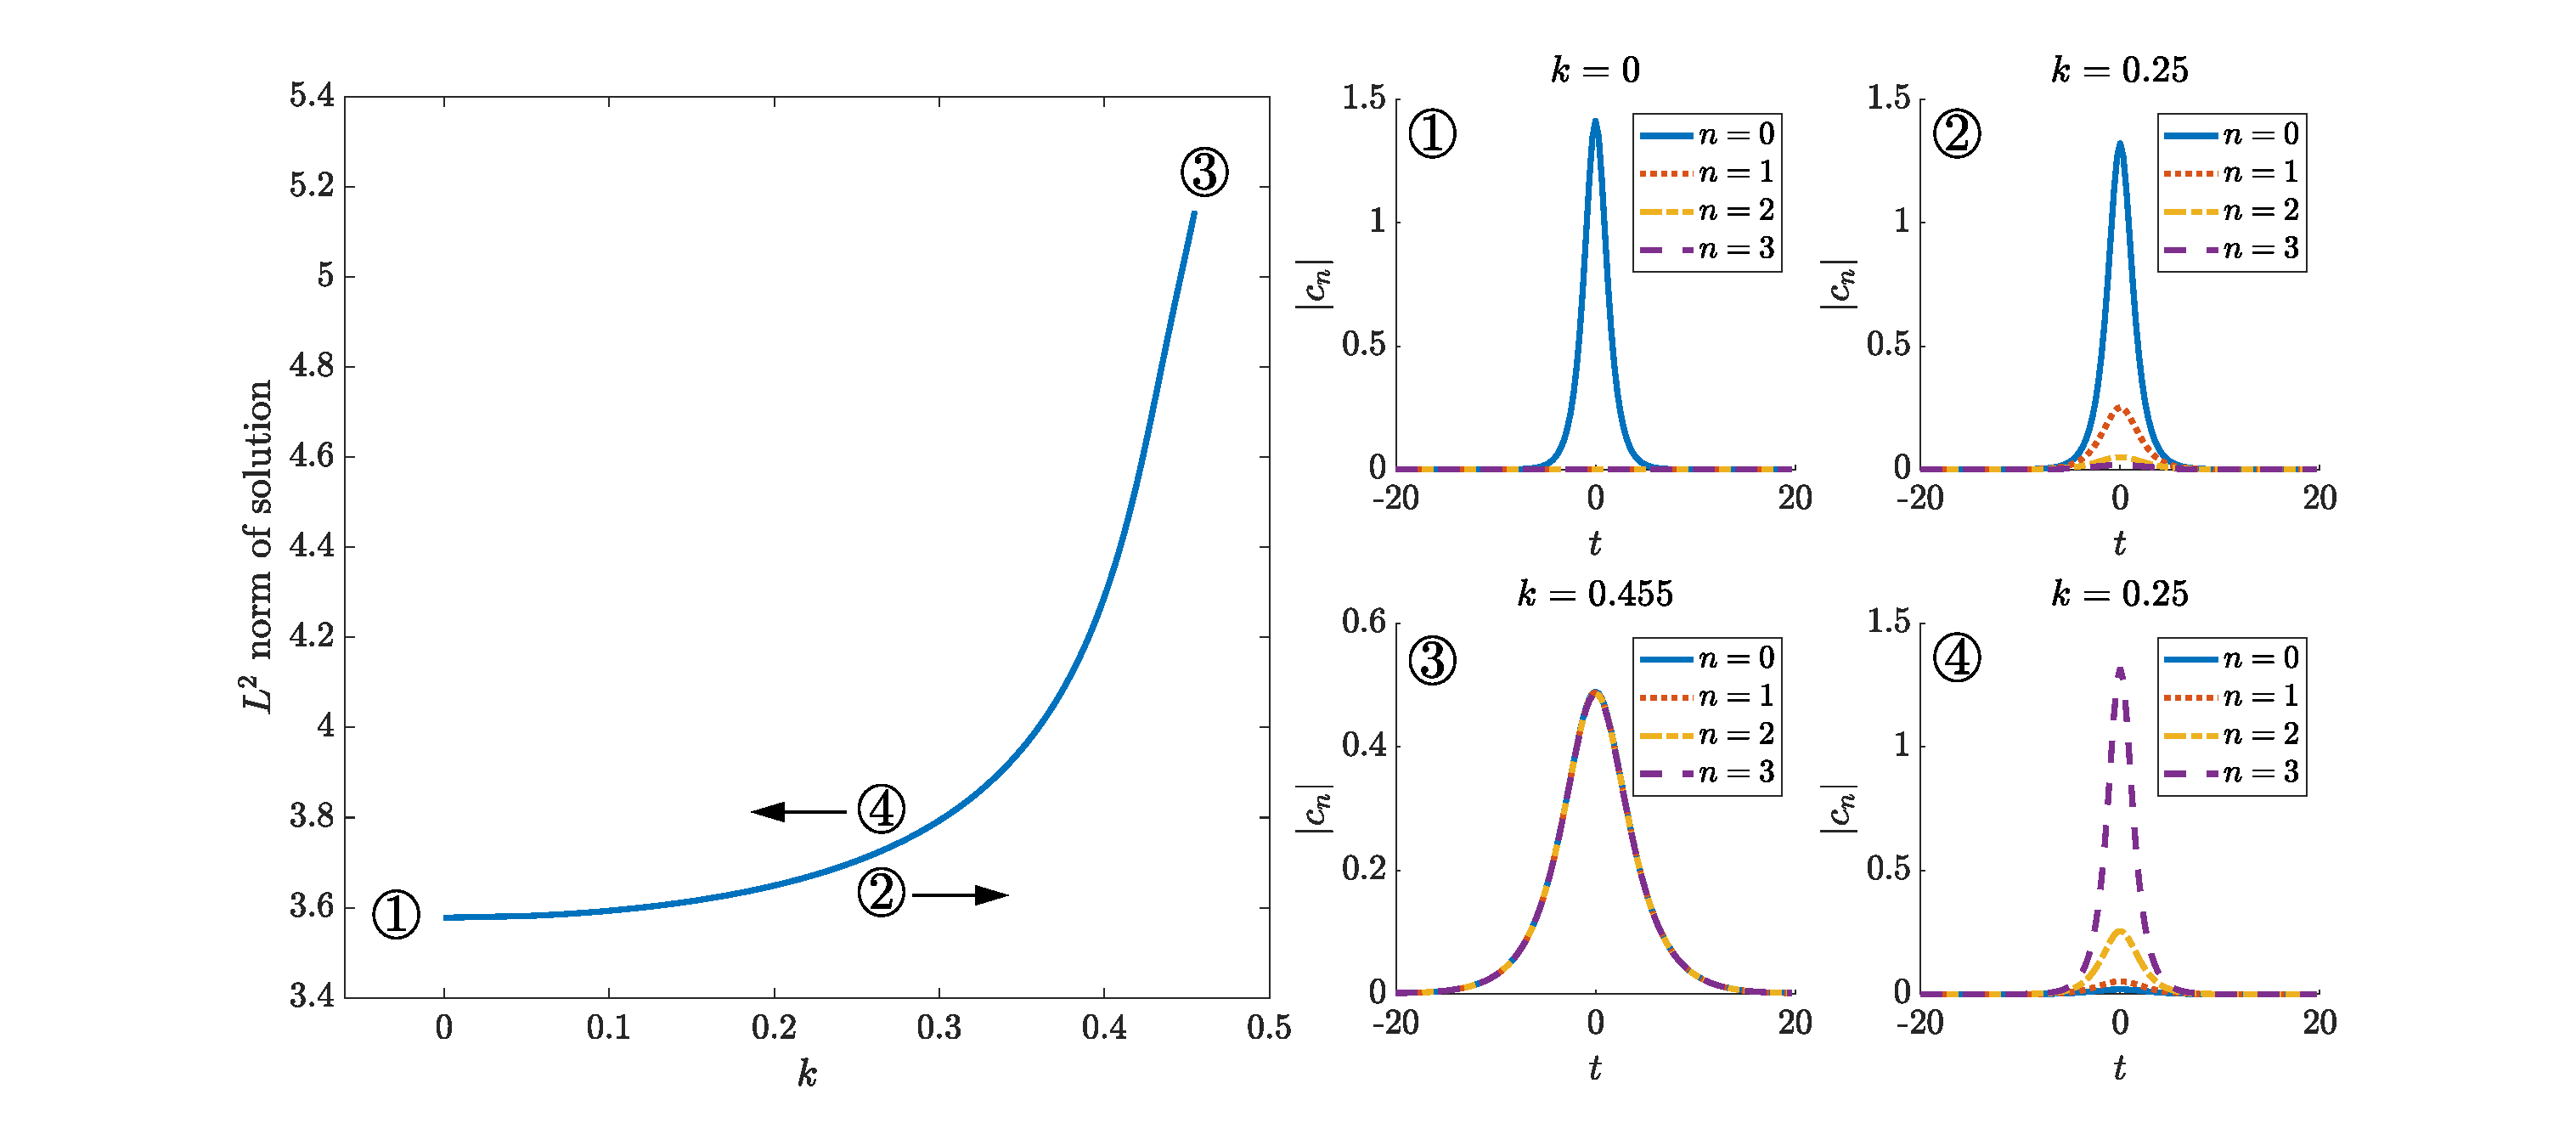
\includegraphics[width=16cm]{contdiag.eps}
    \caption{Parameter continuation in $k$ for solutions to \cref{eq:standingwave} for $\phi=0.25$. Left panel is continuation diagram plotting $L^2$ norm of solution vs. $k$. Right panels show amplitudes of first four sites of representative solutions, which correspond to labeled points on the continuation diagram. Label 2 is $k=0.25$ in the direction of increasing $k$. Label 4 is $k=0.25$ in the direction of decreasing $k$. $\omega=1$, time domain $[-20,20]$, 128 Fourier nodes per core.}
    \label{fig:kcont}
\end{figure}

\begin{figure}
    \centering
    \begin{subfigure}{0.3\linewidth}
        \caption{}
        \label{fig:kcont2q}
        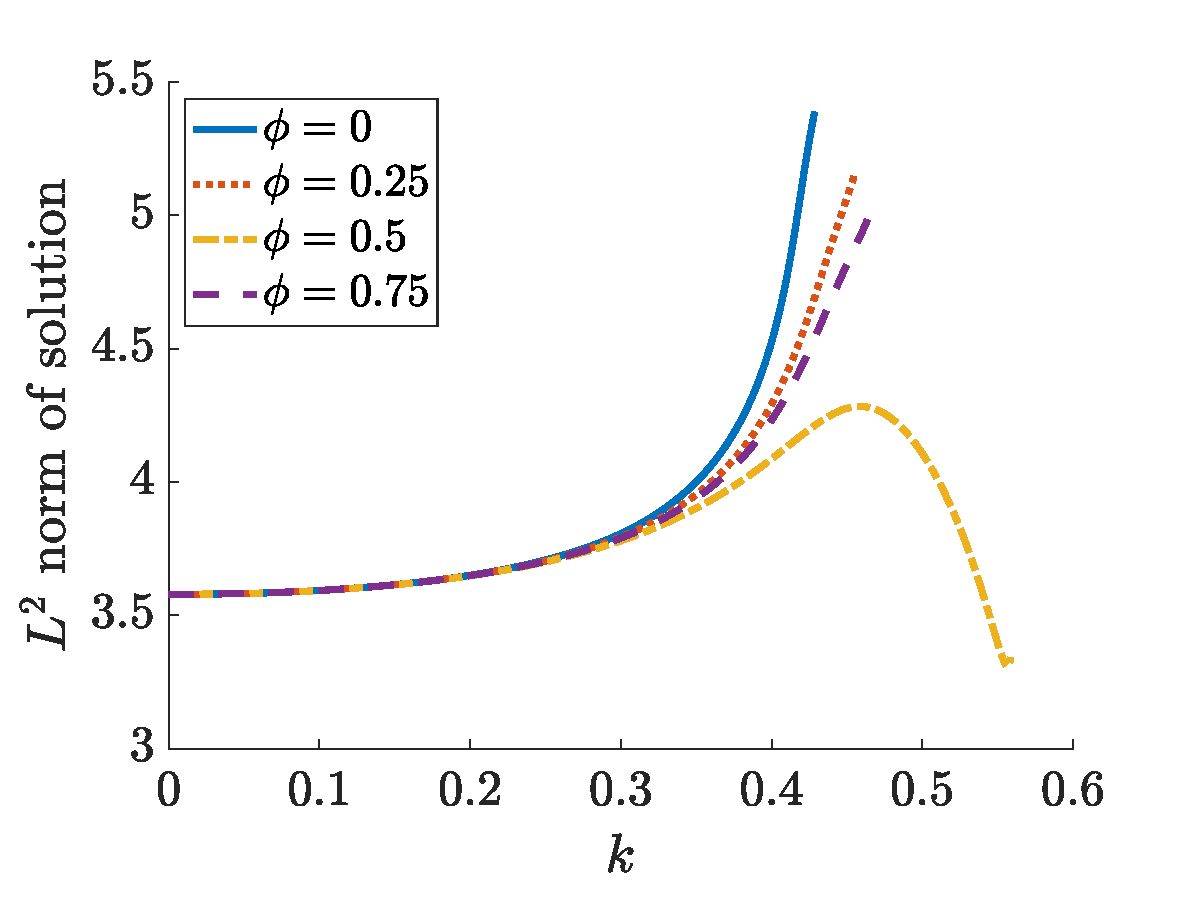
\includegraphics[width=5cm]{contkL2norm.eps}
    \end{subfigure}
    \begin{subfigure}{0.3\linewidth}
        \caption{}
        \label{fig:kcont2b}
        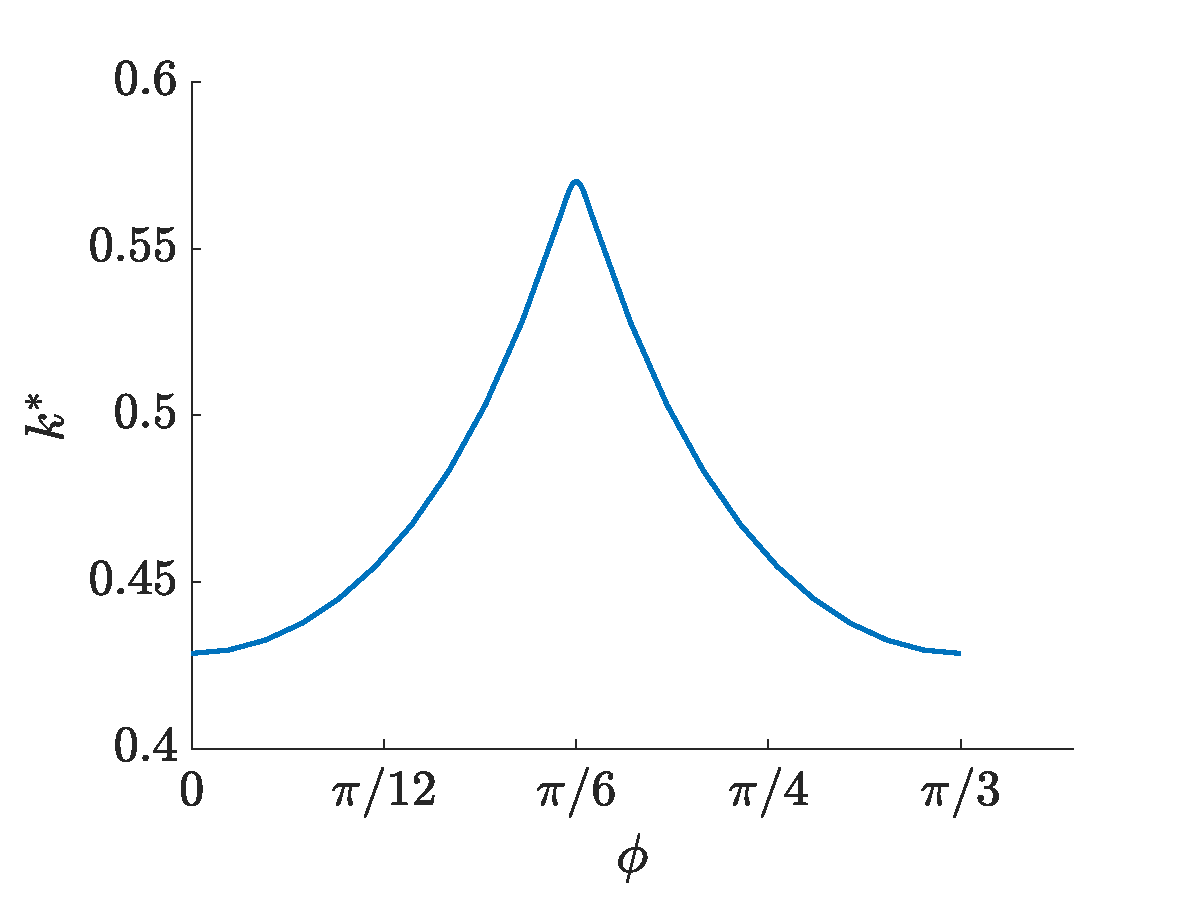
\includegraphics[width=5cm]{contkstarvsphi.eps}
    \end{subfigure}
    \begin{subfigure}{0.3\linewidth}
        \caption{}
        \label{fig:kcont2c}
        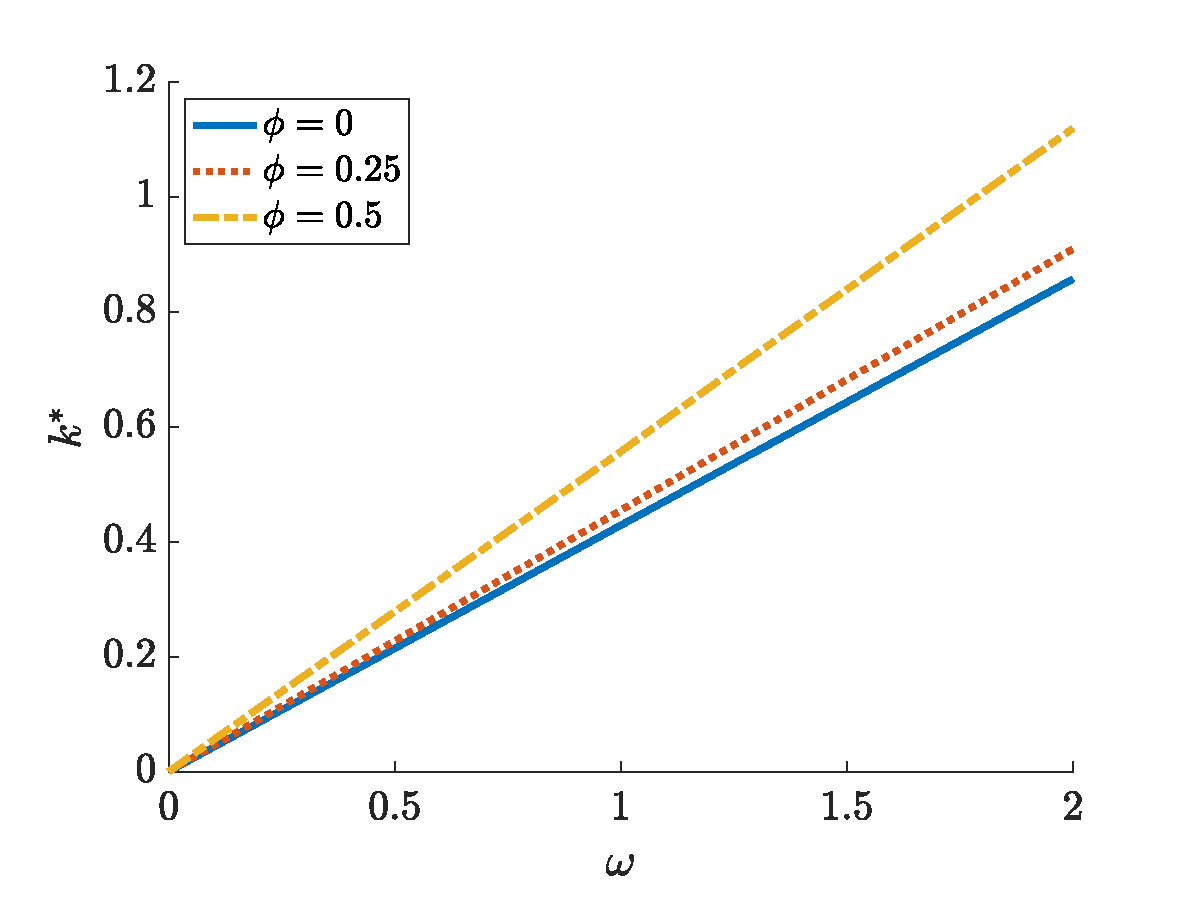
\includegraphics[width=5cm]{contkstarvsomega.eps}
    \end{subfigure}
    \caption{Parameter continuation in $k$ for solutions to \cref{eq:standingwave}. (a) Continuation diagram plotting $L^2$ norm of solution vs. $k$ for various $\phi$. (b) Plot of critical value $k^*$ vs. $\phi$ for $\omega = 1$. (c) Plot of critical value $k^*$ vs $\omega$ for various $\phi$. Time domain $[-20,20]$, 128 Fourier nodes per core.}
    \label{fig:kcont2}
\end{figure}

Results for $N=6$ cores are shown in \cref{fig:m6sol}. As predicted, when $\phi=\pi/6$, there is significant suppression of the amplitude at the opposite site in the ring (\cref{fig:m6pi6logamp}); in addition, we can see from \cref{fig:m6pi6phase} that the lowest order remainder term $\tilde{\phi}_n(t)$ is 0 for the phases $\phi_n(t)$. \cref{fig:m6supp} shows this suppression as $\phi$ is varied, both for the amplitude $a_3(t)$ of the opposite core and the deviations $\phi_n(t) - n \phi$ of the angles.

% figure: amplitudes/phases for N=6
\begin{figure}
    \centering
    \begin{subfigure}{0.3\linewidth}
        \caption{}
        \label{fig:m6025amp}
        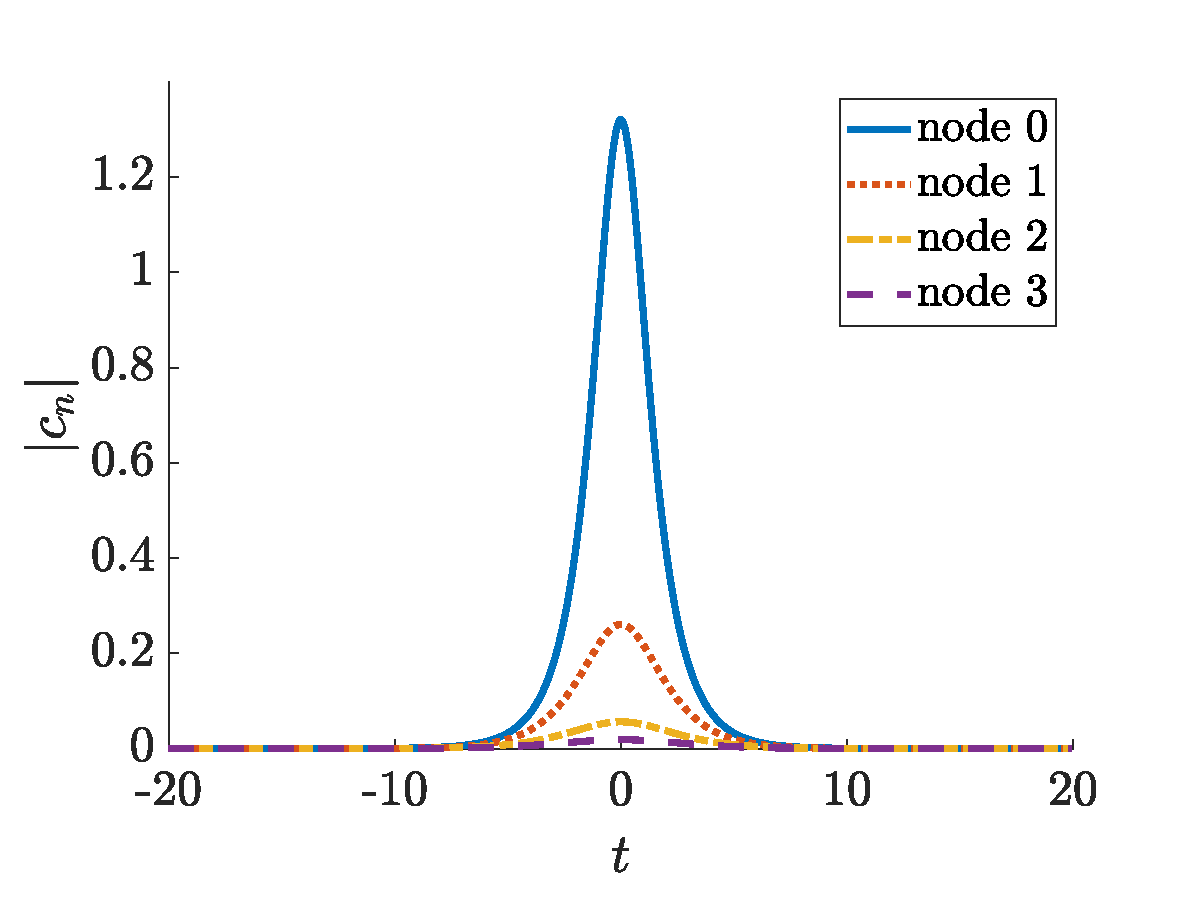
\includegraphics[width=5cm]{m6phi025amp.eps}
    \end{subfigure}
    \begin{subfigure}{0.3\linewidth}
        \caption{}
        \label{fig:m6025logamp}
        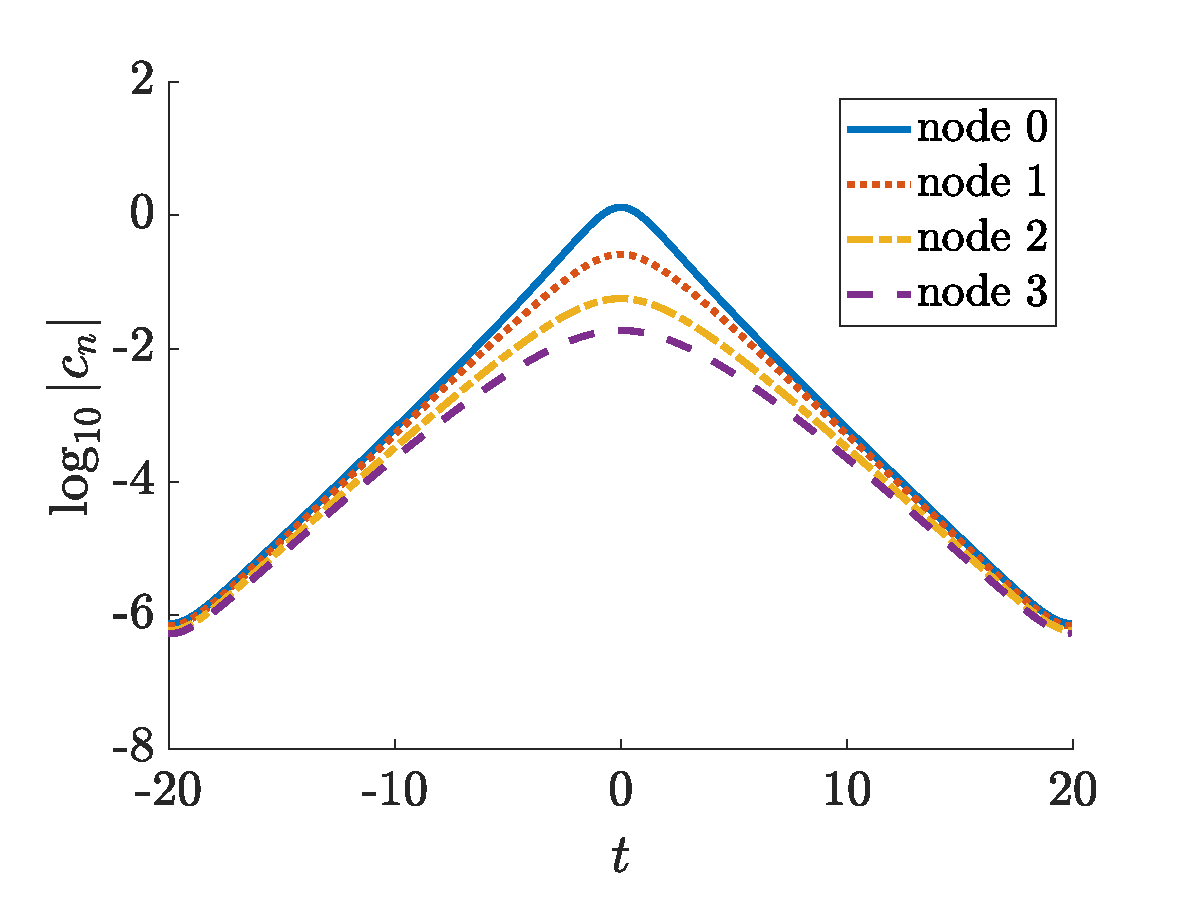
\includegraphics[width=5cm]{m6phi025logamp.eps}
    \end{subfigure}
    \begin{subfigure}{0.3\linewidth}
        \caption{}
        \label{fig:m6025phase}
        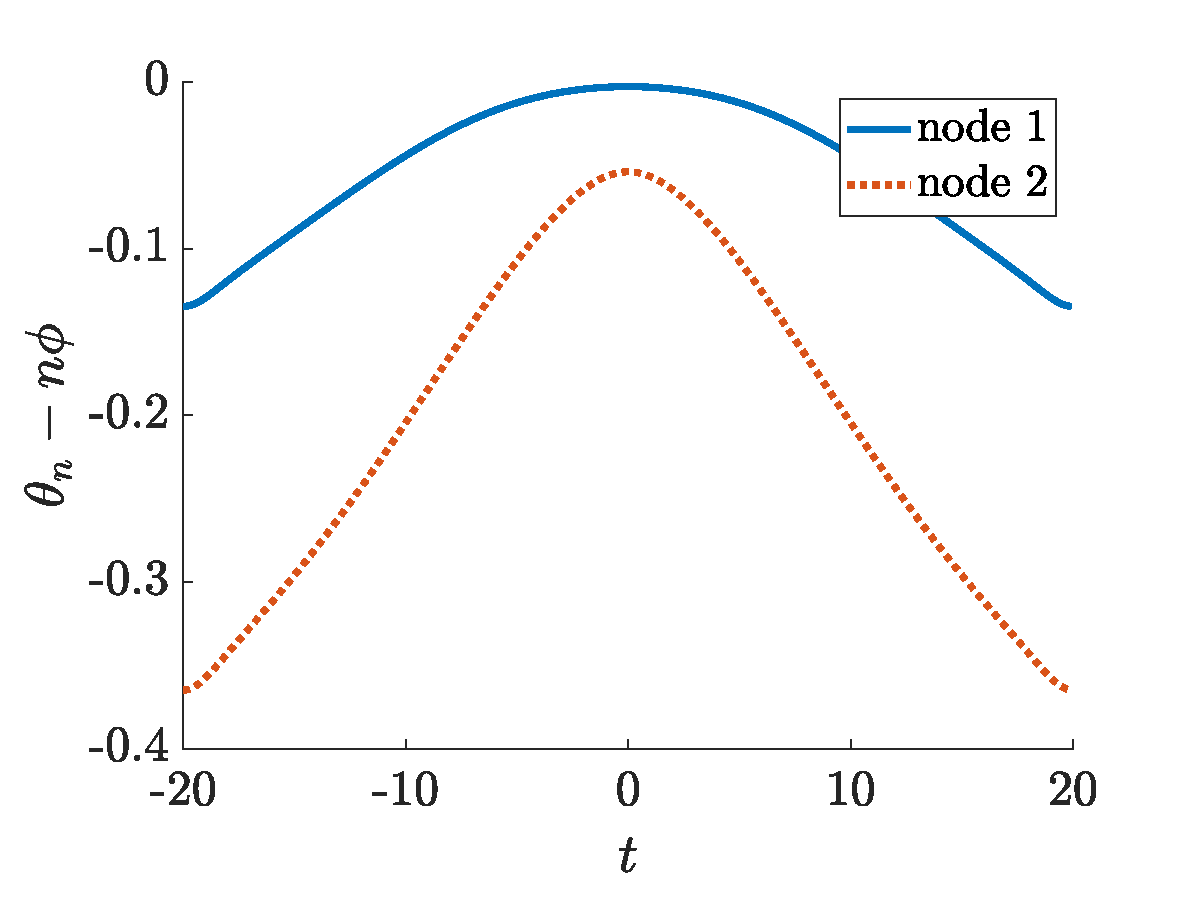
\includegraphics[width=5cm]{m6phi025phase.eps}
    \end{subfigure}
    \begin{subfigure}{0.3\linewidth}
        \caption{}
        \label{fig:m6pi6amp}
        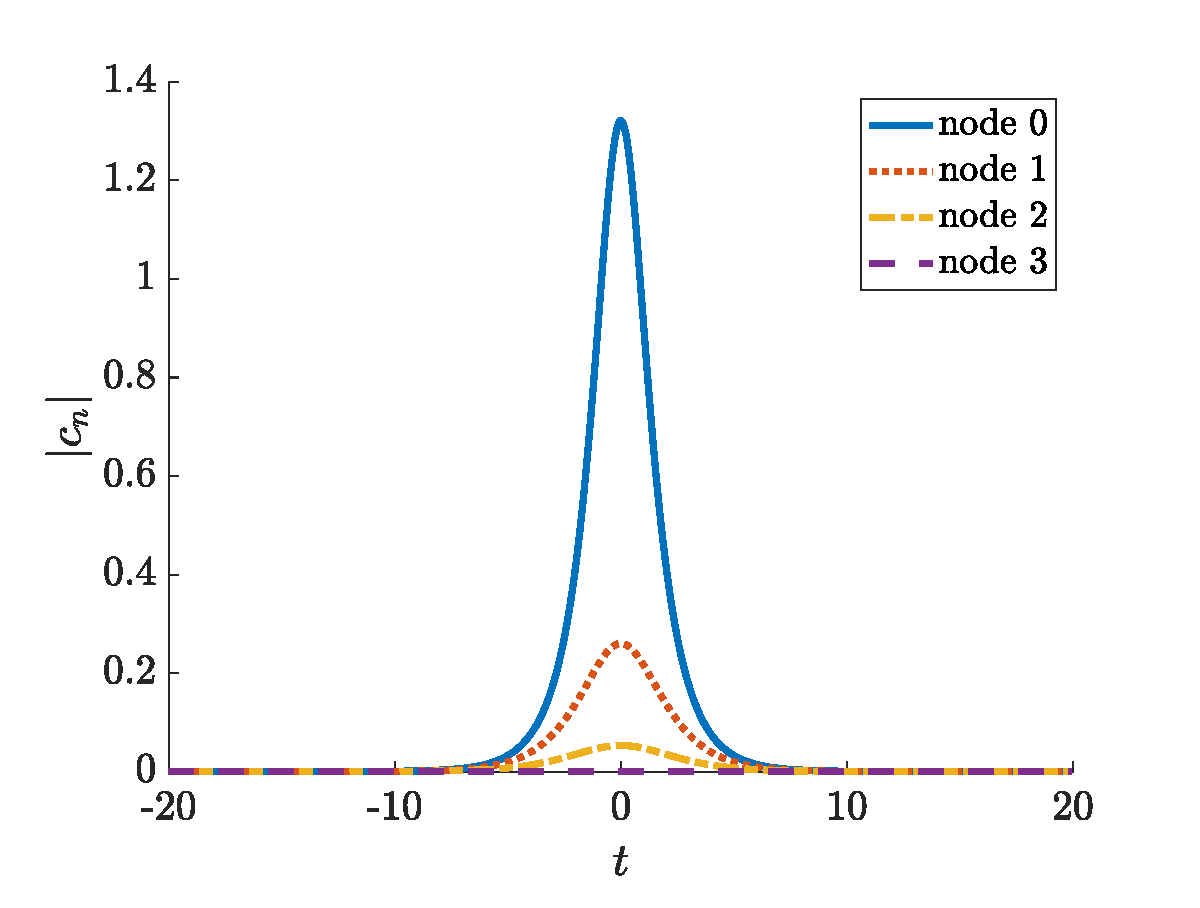
\includegraphics[width=5cm]{m6phipi6amp.eps}
    \end{subfigure}
    \begin{subfigure}{0.3\linewidth}
        \caption{}
        \label{fig:m6pi6logamp}
        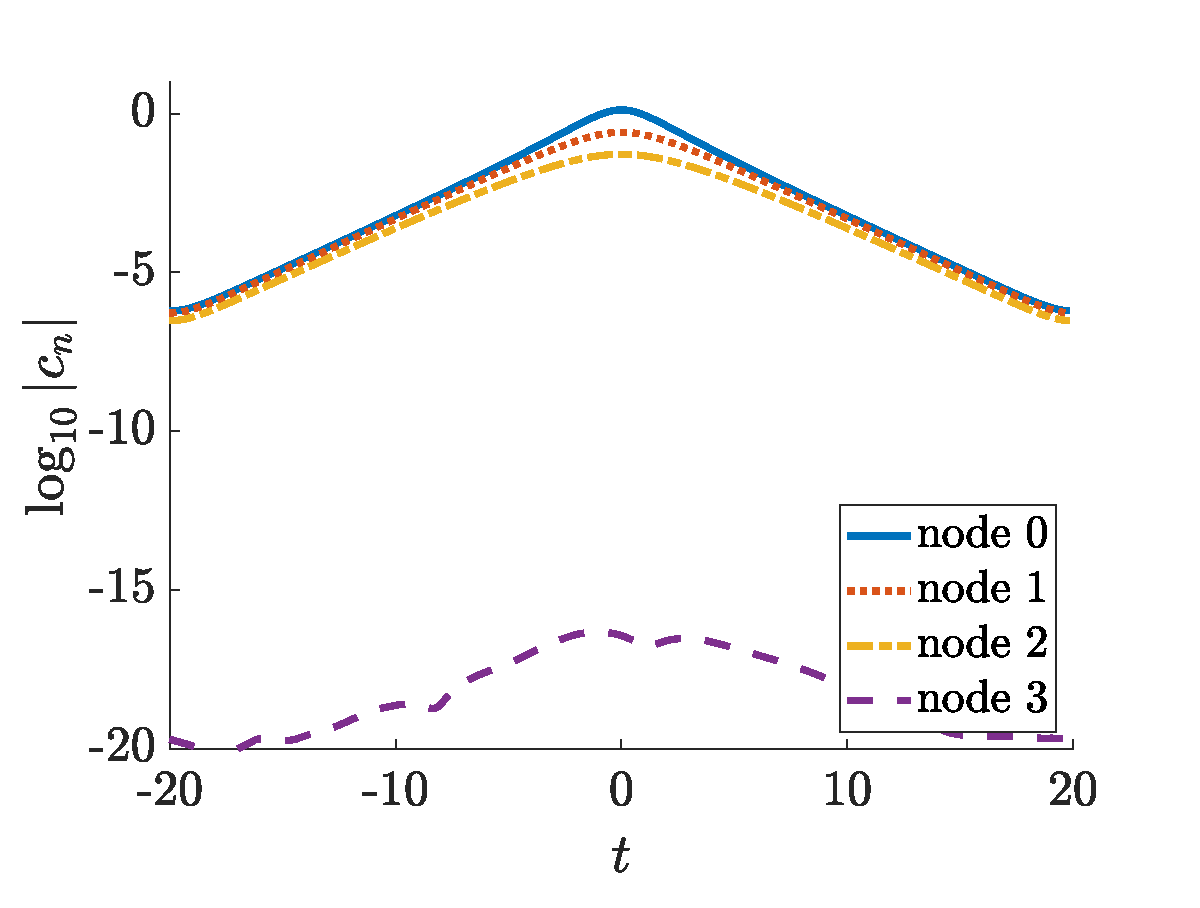
\includegraphics[width=5cm]{m6phipi6logamp.eps}
    \end{subfigure}
        \begin{subfigure}{0.3\linewidth}
        \caption{}
        \label{fig:m6pi6phase}
        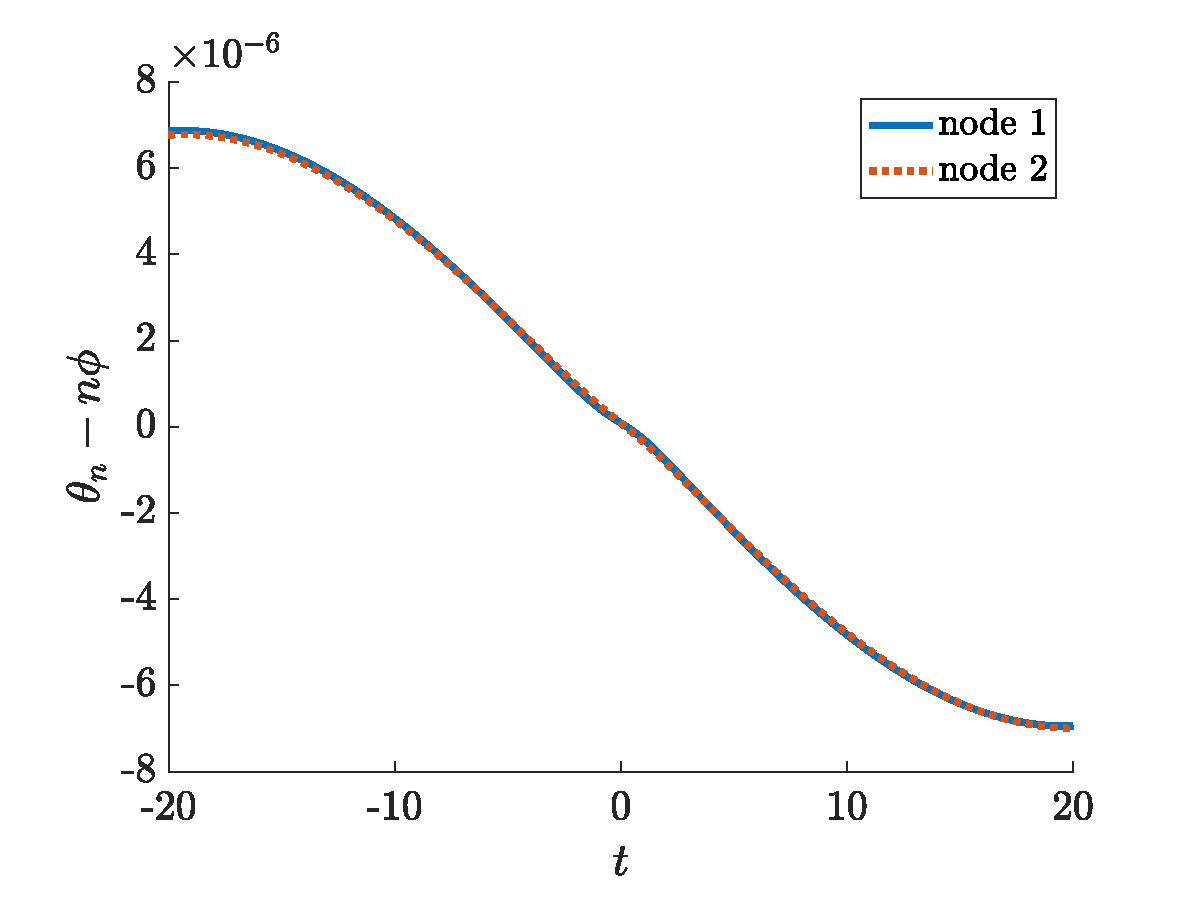
\includegraphics[width=5cm]{m6phipi6phase.eps}
    \end{subfigure}
    \caption{Standing wave solutions to equation \cref{eq:standingwave} for $N=6$ waveguides. Twist parameter $\phi = 0.25$ (top), $\phi = \pi/6$ (bottom). Left and middle are amplitude and log amplitude of solution at first four sites. Right plots $\theta_n(t) - n \phi$ for sites 1 and 2, where $\theta_n(t)$ is the phase. $k=0.25$, $\omega=1$, time domain $[-30,30]$, 256 Fourier nodes per core.}
    \label{fig:m6sol}
\end{figure}

% figure: amplitudes/phases for N=6
\begin{figure}
    \centering
    \begin{subfigure}{0.4\linewidth}
        \caption{}
        \label{fig:m6suppa3}
        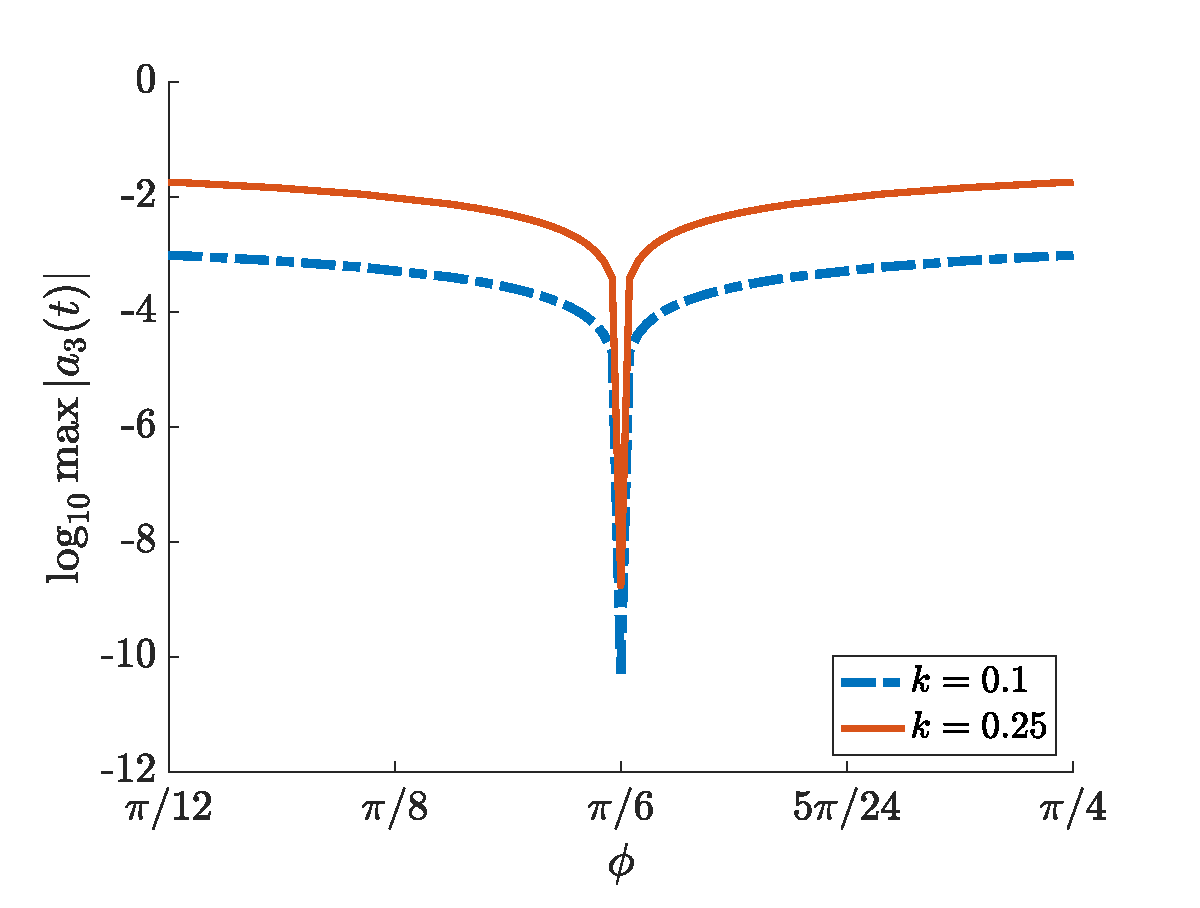
\includegraphics[width=5cm]{a3phicont.eps}
    \end{subfigure}
    \begin{subfigure}{0.4\linewidth}
        \caption{}
        \label{fig:m6supptheta}
        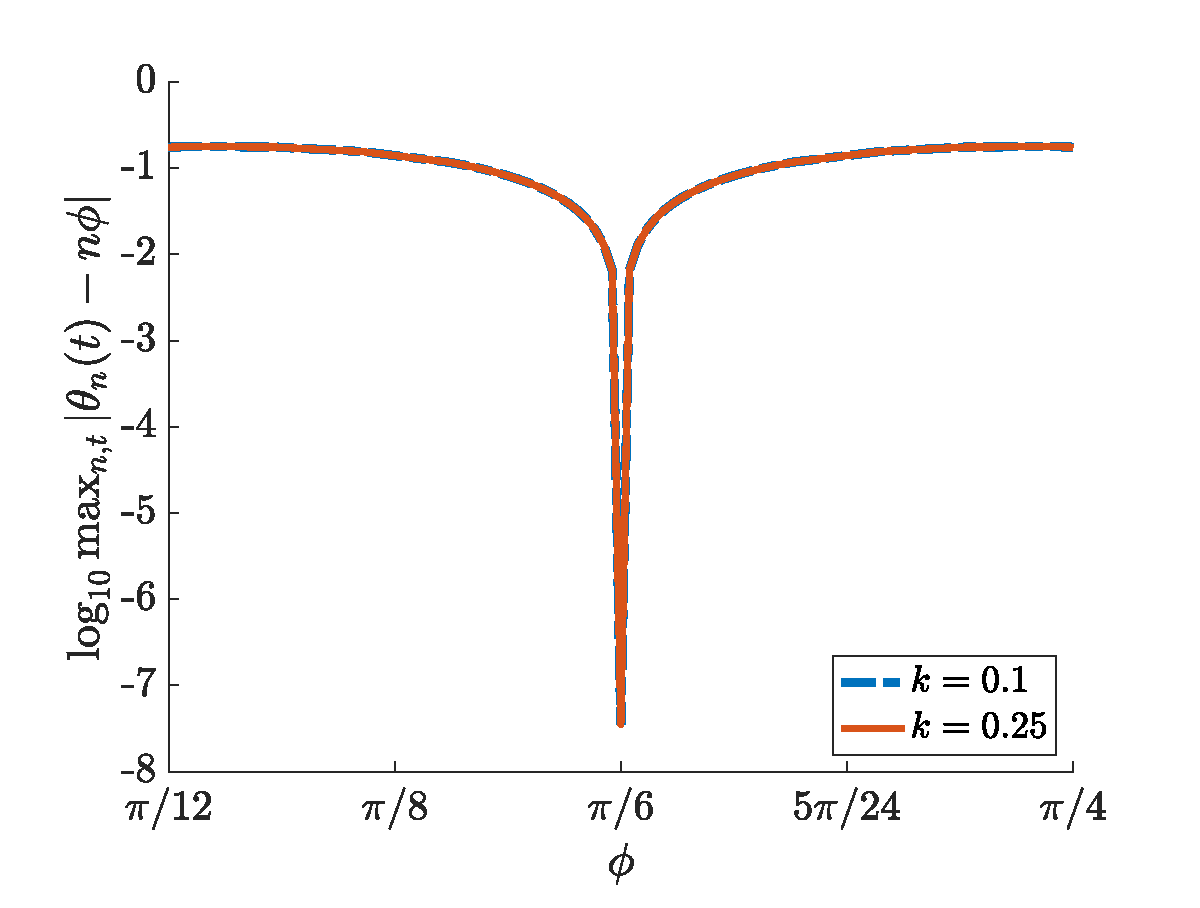
\includegraphics[width=5cm]{thetaphicont.eps}
    \end{subfigure}
    \caption{(a) $\log_{10} \max |a_3(t)|$ vs. $\phi$ for $k=0.1$ and $k=0.25$. (b) $\log_{10} \max_{n,t}{|\theta_n(t) - n \phi|}$ vs. $\phi$ for $k=0.1$ and $k=0.25$.}
    \label{fig:m6supp}
\end{figure}

Next, we compute the error in for the amplitudes $a_n(t)$ and phases $\theta_n(t)$. \cref{fig:m6errora} plots the log of the $L^2$ error $\| a_n^{\text{true}}(t) - a_n^{\text{approx}}(t) \|_{L^2}$ vs. the log of coupling parameter $k$, where the true value $a_n^{\text{true}}(t)$ is obtained from numerical parameter continuation, the approximate value $a_n^{\text{approx}}(t)$ is computed using \cref{eq:asympsol}, \cref{eq:tildeanpsi}, and \cref{eq:tildea0eq}, and the $L^2$ norm on the periodic domain $[-T,T]$ is defined by
\[
\| f(t) \|_{L^2} = \int_{-T}^T |f(t)|^2 dt.
\] 
The slopes of least squares regressions lines for the error in $a_0(t)$, $a_1(t)$, $a_2(t)$, and $a_3(t)$ are within 5\% of 4, 3, 4, and 5 (respectively), which suggests that the asymptotic expansions \cref{eq:asympsol} for the amplitudes are, in fact, 
\begin{equation}\label{eq:asympsol2}
\begin{aligned}
a_0(t) &= \psi(t) + k^2 \tilde{a}_0(t) + \mathcal{O}(k^4) \\
a_n(t) &= k^n \tilde{a}_n(t) + \mathcal{O}(k^{n+2}) && n = 1, \dots, N/2
\end{aligned}
\end{equation}
i.e. the order of the remainder term is one order higher in $k$. Since the formulas \cref{eq:tildeantnpsi} involve the products $a_n(t) \theta_n(t)$ of the amplitudes and phases, \cref{fig:m6errorb} plots the log of the $L^2$ error of $\| (a_n(t) (\theta_n(t) - n \phi)^{\text{true}} - (a_n(t) \theta_n(t)- n \phi)^{\text{approx}}(t) \|_{L^2}$ vs. the log of coupling parameter $k$, where the true value is obtained from numerical parameter continuation, and the approximate value is computed using 
$a_n(t) \theta_n(t) - n \phi )^{\text{approx}}(t) = k^{N-n} \tilde{a}_n(t) \tilde{\theta}_n(t)$ and \cref{eq:tildeantnpsi}. The slopes of least squares regressions lines for the error in $a_1(t)\theta_1(t)$ and $a_2(t)\theta_2(t)$ are within 2.5\% of 5 and 4 (respectively), which suggests that the order of the remainder term in $k$ is correct in the asymptotic expansions \cref{eq:asympsol} for $\theta_n(t)$.

% figure: amplitudes/phases for N=6
\begin{figure}
    \centering
    \begin{subfigure}{0.4\linewidth}
        \caption{}
        \label{fig:m6errora}
        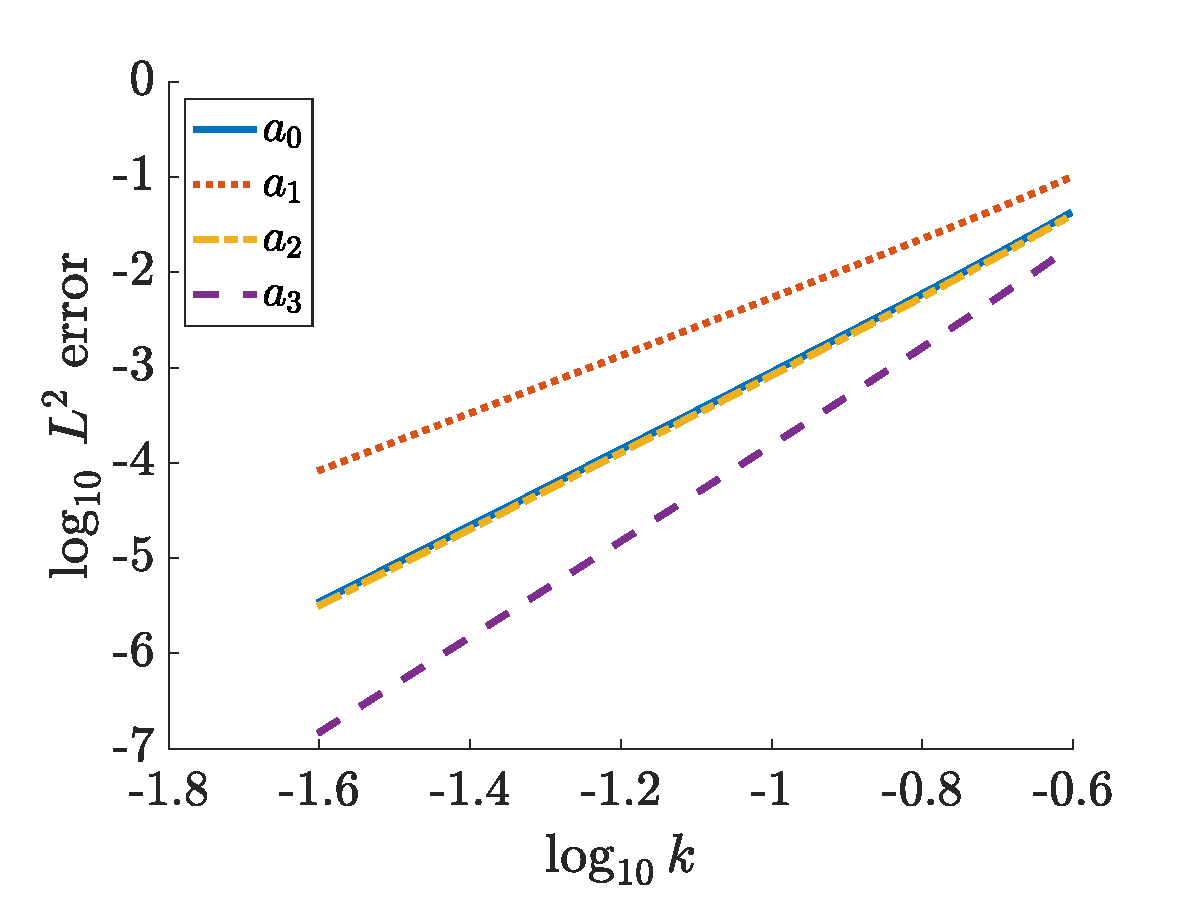
\includegraphics[width=5cm]{N6aerror.eps}
    \end{subfigure}
        \centering
    \begin{subfigure}{0.4\linewidth}
        \caption{}
        \label{fig:m6errorb}
        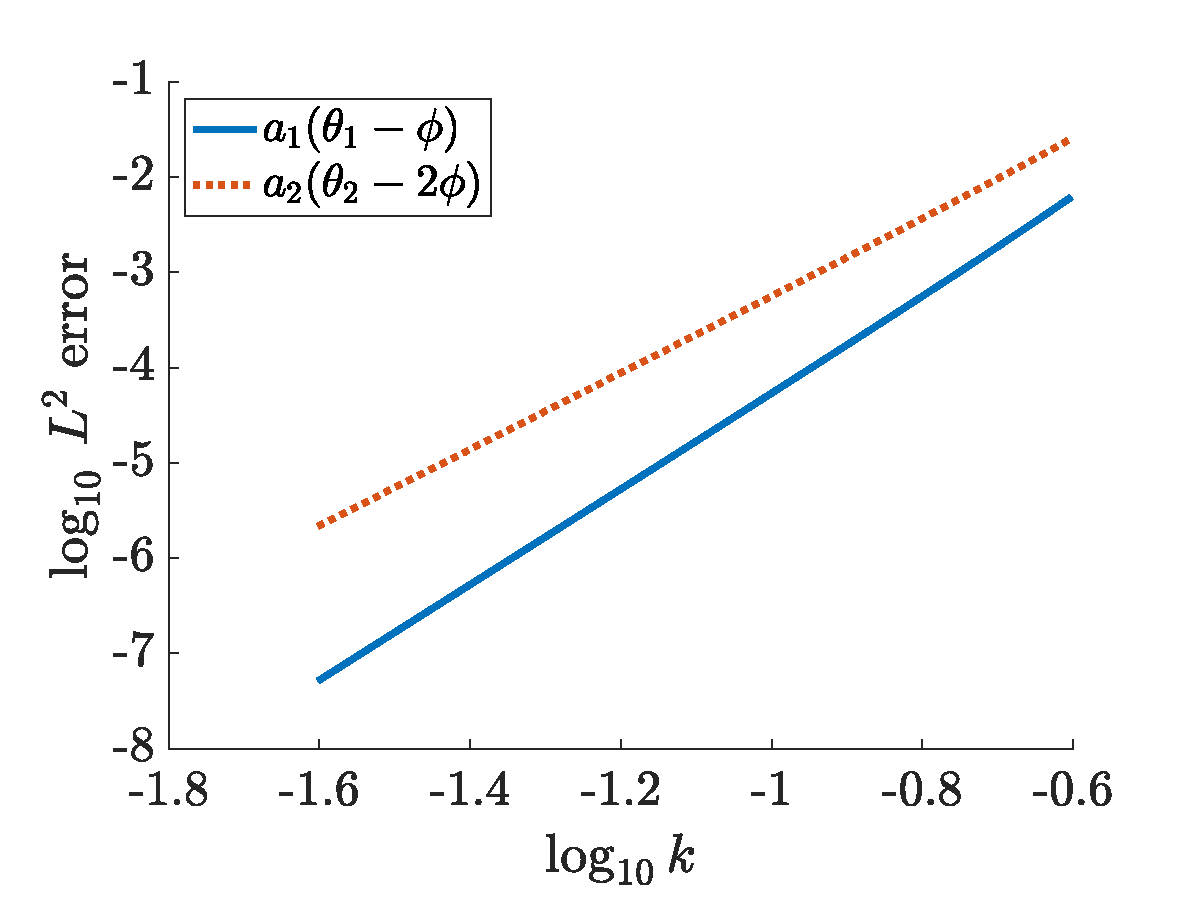
\includegraphics[width=5cm]{N6athetaerror.eps}
    \end{subfigure}
    \caption{$\log_{10}$ of $L^2$ error of the amplitudes $a_n(t)$ vs $\log_{10} k$ (a), and the product of the amplitudes and phases $a_n(t)\theta_n(t)$ vs $\log_{10} k$.}
    \label{fig:m6error}
\end{figure}


\section{Stability}\label{sec:stability}

Let $c = (c_1, \dots, c_n)$ be a solution to \cref{eq:standingwavematrix}. This time, we split up the $c_n$ into real and imaginary parts by writing $c_n = u_n + i v_n$ for $n = 1, \dots, N$. The linearization of the PDE \cref{eq:cz} about the standing wave $c$ is the linear operator $\calL(c)$ on $H^2(\R, \R^{2N}) \subset L^2(\R, \R^{2N})$, defined by 
\begin{equation}\label{eq:linc}
\calL(c) = \begin{pmatrix}
k A_i(\phi) + 2 \diag(u_n v_n) & \partial_t^2 - \omega + k A_r(\phi) + \diag(u_n^2) + 3 \diag(v_n^2) \\
-\partial_t^2 + \omega - k A_r(\phi) - 3\diag(u_n^2) - \diag(v_n^2) &
k A_i(\phi) - 2 \diag(u_n v_n)
\end{pmatrix},
\end{equation}
where
\begin{align*}
A_r(\phi) &= \text{Re } A(\phi) = \begin{pmatrix}
0 & \cos \phi & & \dots & \cos \phi \\
\cos \phi & 0 & \cos \phi & & & \\
& \ddots & \ddots & \ddots &  & \\
 & &\cos \phi  & 0 & \cos \phi  \\
\cos \phi& \dots & & \cos \phi & 0
\end{pmatrix} \\
A_i(\phi) &= \text{Im } A(\phi) = \begin{pmatrix}
0 & -\sin \phi & & \dots & \sin \phi \\
\sin \phi & 0 & -\sin \phi & & & \\
& \ddots & \ddots & \ddots &  & \\
 & &\sin \phi  & 0 & -\sin \phi  \\
-\sin \phi& \dots & & \sin \phi & 0
\end{pmatrix}.
\end{align*}
The kernel of $\calL(c)$ is spanned by the two eigenfunctions 
$w_1 = (\partial_t u_1, \dots, \partial_t u_N, \partial_t v_1, \dots, \partial_t v_N )^T$ and 
$w_2 = (-v_1, \dots, -v_N, u_1, \dots, u_N )^T$.

\appendix

\section{Symmetries}\label{app:symm}

We verify that the symmetry relations in \cref{eq:symm} are consistent. First, for $n = 2, \dots, N/2-1$, we take equation \cref{eq:st2} for $-n$, substitute the symmetries for $a_n$ and $\theta_n$ from \cref{eq:symm}, and simplify, to obtain 
\begin{equation*}
\begin{aligned}
(\ddot a_n &- a_n (\dot \theta_n)^2) 
- i ( a_n \ddot\theta_n + 2 \dot a_n \dot \theta_n )\\
&+ k\left(a_{n-1}e^{i[(\theta_n - \theta_{n-1}) - \phi]} + a_{n+1}e^{-i[(\theta_{n+1} - \theta_{n}) - \phi]} \right)+a_n^3 - \omega a_n = 0,
\end{aligned}
\end{equation*}	
which is the complex conjugate of \cref{eq:st2} for $n$. For $n = 0$, we take equation \cref{eq:st2} for $n=0$, substitute the symmetries for $a_n$ and $\theta_n$ from \cref{eq:symm}, and simplify, to obtain 
\begin{equation*}
\begin{aligned}
(\ddot a_0 &- a_0 (\dot \theta_0)^2) 
+ i ( a_0 \ddot\theta_0 + 2 \dot a_0 \dot \theta_0 )
+ 2 k a_1 \cos(\theta_1 - \phi)(\cos \theta_0 + i \sin \theta_0) + a_n^3 - \omega a_n = 0.
\end{aligned}
\end{equation*}
The imaginary part is
\begin{equation}\label{eq:n0imagpart}
a_0 \ddot\theta_0 + 2 \dot a_0 \dot \theta_0 = 2 k a_1 \cos(\theta_1 - \phi) \sin \theta_0,
\end{equation}
for which $\theta_0(t) = 0$ is a solution, thus this condition is consistent. Following the same procedure by using the imaginary part of equation \cref{eq:st2}, we can show that the $\theta_{N/2} = 0$ is a solution to the imaginary part of \cref{eq:st2} for $n=N/2$, thus this condition is consistent as well.

\section{Asymptotics}\label{app:asymp}

Let $a_n(t)$ and $\theta_n(t)$ be the amplitudes and phases at site $n$, as in the ansatz \cref{eq:cnansatz}, where $n \in S = \{ 0, \pm 1, \dots, \pm N/2-1, N/2 \}$. We will take 
\[
a_n(t), \theta_n(t) \in H^2(\R) \subset L^2(\R),
\]
where $L^2(\R)$ is the space of real, valued square-integrable functions on $\R$ equipped with the standard inner product, and $H^2(\R)$ is the corresponding Sobelev space. We note that the system of equations \cref{eq:st2} is translation invariant, i.e. if $\{ a_n(t), \theta_n(t)\}_{n\in S}$ is a solution, then so is $\{ a_n(t-\tau), \theta_n(t-\tau)\}_{n\in S}$ for any $\tau \in \R$. When $k = 0$, we want the solution $a_0(t)$ to be the ordinary NLS soliton $\psi(t)$, which is centered at 0. To ensure that the solution we find is not shifted in $t$, we impose the phase condition on the amplitude $a_0(t)$
\begin{equation}\label{eq:phasecond}
\langle a_0(t), \dot{\psi}(t) \rangle_{L^2(\R)} = \int_{-\infty}^\infty a_0(t) \dot{\psi}(t) dt = 0.
\end{equation}
In other words, $a_0(t)$ will have no component in the direction of $\dot{\psi}(t)$.

Next, define the linear operator $\Lw: H^2(\R) \subset L^2(\R) \rightarrow L^2(\R)$ by
\begin{equation}\label{eq:Lw}
\Lw = \omega - \partial_t^2.
\end{equation}
Since all functions in $L^2(\R)$ vanish at infinity, the kernel of $\Lw$ is $\{0\}$, i.e. the only solution in $H^2(\R)$ to $\Lw f = 0$ is $f = 0$. Furthermore the operator $\Lw$ is invertible [REF?].

Finally, we recall that the NLS soliton $\psi(t)$ is a real-valued, standing wave solution to the NLS equation with frequency $\omega$, thus it solves 
\begin{equation}\label{eq:NLSreal}
\ddot{u} + u^3 - \omega u = 0. 
\end{equation}
Linearizing this equation about $\dot{\psi}(t)$ yields the self-adjoint linear operator $\calL(\psi): H^2(\R) \subset L^2(\R) \rightarrow L^2(\R)$, defined by
\begin{equation}\label{eq:Lpsi}
\calL(\psi) = \partial_t^2 - \omega + 3 \psi^2.
\end{equation}
The kernel of $\dot{\psi}(t)$ is one-dimensional, and is spanned by $\{ \dot{\psi}(t) \}$. By the Fredholm alternative [REF], since $\calL(\psi)$ is self-adjoint, the equation $\calL(\psi) = u(t)$ has a solution if $u(t) \perp \dot{\psi}(t)$.

\subsection{Primary core}

Using the symmetry relations \cref{eq:symm} and $\theta_0(t) = 0$, equation \cref{eq:st2real} for $n=0$ becomes
\begin{equation}\label{eq:st2reala0}
\ddot a_0  + 2 k a_1 \cos(\theta_1 - \phi) + a_0^3 - \omega a_0 = 0 
\end{equation}
We take the power series ansatz 
\[
a_0(t) = \psi(t) + k a_0^{(1)}(t) + k^2 a_0^{(2)}(t) + \mathcal{O}(k^3)
\]
for the amplitude $a_0(t)$, where $\psi(t)$ is the NLS soliton \cref{eq:NLSsoliton}. In addition, from \cref{eq:basicseries}, we have, at minimum, 
\[
a_1(t) = k \tilde{a}_1(t) + \mathcal{O}(k^2), \qquad \theta_1(t) = \phi + \mathcal{O}(k).
\]
Substituting this into \cref{eq:st2reala0}, using the Taylor series expansion $\cos(\theta_1-\phi) = \mathcal{O}(k^2)$, collecting powers of $k$, and simplifying, we get
\begin{equation*}
\begin{aligned}
&\left(\ddot{\psi} + \psi^3 - \omega \psi\right) 
+ k\left(\ddot a_0^{(1)} - \omega a_0^{(1)} + 3 \psi^2 a_0^{(1)}\right) \\
&\qquad\qquad+ k^2\left(\ddot a_0^{(2)} - \omega a_0^{(2)} + 3\left(a_0^{(1)}\right)^2 + 3 \psi^2 a_0^{(2)} + 2 \tilde{a}_1 \right) + \mathcal{O}(k^3) = 0,
\end{aligned}
\end{equation*}
where we have dropped the dependence on $t$ for simplicity. The $\mathcal{O}(1)$ term is 0 since $\psi$ solves \cref{eq:NLSreal}. The $\mathcal{O}(k)$ term can be written as $\calL(\psi)a_0^{(1)}=0$, where $\calL(\psi)$ is defined by \cref{eq:Lpsi}. Since the kernel of $\calL(\psi)$ is spanned by $\dot \psi(t)$, $a_0^{(1)} = c \dot \psi(t)$ for some constant $c$. However, since we wish our solution to satisfy the phase condition \cref{eq:phasecond}, we will take $c = 0$, from which it follows that $a_0^{(1)} = 0$. The $\mathcal{O}(k^2)$ term then becomes
\[
\ddot a_0^{(2)} - \omega a_0^{(2)} + 3 \psi^2 a_0^{(2)} + 2 \tilde{a}_1 = 0.
\]
Letting $\tilde{a}_0(t) = a_0^{(2)}(t)$, we rewrite this as
\begin{align}\label{eq:solvea0ta}
\calL(\psi) \tilde{a}_0 = -2 \tilde{a}_1.
\end{align}
Once we determine $\tilde{a}_1$, which we will do in the next step, we can solve for $\tilde{a}_0$, provided $\tilde{a}_1 \perp \dot\psi$. Putting all of this together, we have the expression for $a_0$
\begin{equation}\label{eq:a0eq}
a_0(t) = \psi(t) + k^2 \tilde{a}_0(t) + \mathcal{O}(k^3) = \psi(t) + \mathcal{O}(k^2).
\end{equation}

\subsection{Amplitudes}

We can now determine the leading order terms for the amplitudes $a_n$, for $n = 1, \dots, N/2$, using the real parts \cref{eq:st2real} of the equations \cref{eq:st2}. The phases $\theta_n$ will be determined in the next step. For $n=1$, we take the power series ansatz 
\[
a_1(t) = k \tilde{a}_1(t) + \mathcal{O}(k^2).
\]
From \cref{eq:basicseries}, we have, at minimum,
\[
a_2(t) = \mathcal{O}(k^2), \qquad \theta_1(t) = \phi + \mathcal{O}(k), \qquad \theta_2(t) = 2 \phi + \mathcal{O}(k),
\]
and we note that $\dot \theta_1(t) = \mathcal{O}(k)$. Substituting these together with the expression \cref{eq:a0eq} for $a_0(t)$ into the $n=1$ equation of \cref{eq:st2real}, expanding the cosine terms in Taylor series, collecting powers of $k$, and simplifying, we obtain the equation
\[
k\left(\partial_t^2 \tilde{a}_1 - \omega \tilde{a}_1 + \psi\right) + \mathcal{O}(k^2) = 0.
\]
We note that the nonlinear term $a_1^3$ does not contribute to the lowest order term in the asymptotic expansion. We use the $\mathcal{O}(k)$ term to solve for $\tilde{a}_1$ to get 
\begin{equation}\label{eq:a11}
\tilde{a}_1(t) = (\omega - \partial_t^2)^{-1} \psi(t),
\end{equation}
which has a solution since $\Lw$ is invertible. This gives us
\begin{equation}\label{eq:a1eq}
a_1(t) = k (\omega - \partial_t^2) \psi(t) + \mathcal{O}(k^2).
\end{equation}

We continue this process iteratively from $n=2$ to $n=N/2-1$. We take the power series ansatz 
\[
a_n(t) = k^n \tilde{a}_n(t) + \mathcal{O}(k^{n+1}),
\]
and use
\begin{align*}
&a_{n-1}(t) = k^{n-1} \tilde{a}_{n-1}(t) + \mathcal{O}(k^{n}), &&a_{n+1}(t) = \mathcal{O}(k^{n+1}), \\
&\theta_{n-1}(t) = (n-1) \phi + \mathcal{O}(k), &&\theta_{n+1}(t) = (n+1) \phi + \mathcal{O}(k),
\end{align*}
where the expression for $a_{n-1}(t)$ was found in the previous step. Substituting these into \cref{eq:st2real} and following the same procedure as above, we obtain the equation
\begin{align*}
k^n\left(\partial_t^2 \tilde{a}_n - \omega \tilde{a}_n + \tilde{a}_{n-1} \right) +\mathcal{O}(k^{n+1}) = 0.
\end{align*}
We use the $\mathcal{O}(k^n)$ term to solve for $\tilde{a}_n$ to get 
\begin{equation}\label{eq:ann}
\tilde{a}_n = (\omega - \partial_t^2)^{-1}\tilde{a}_{n-1},
\end{equation}
which gives us
\begin{equation}\label{eq:aneq}
a_n(t) = k^n (\omega - \partial_t^2)^{-1} \tilde{a}_{n-1}(t) + \mathcal{O}(k^{n+1}).
\end{equation}
We note that it follows from the ansatz $\theta_n = n \phi + \mathcal{O}(k)$ that $\cos[(\theta_n - \theta_{n-1}) - \phi] = 1 + \mathcal{O}(k^2)$ for all $n$, i.e. all the cosine terms are 1 to leading order. 

For the final node $n=N/2$, we take $\theta_{N/2}(t) = 0$ in the real part of \cref{eq:st2} for $n = N/2$, use the symmetry relations for $a_{N/2-1}$ and $\theta_{N/2-1}$ from \cref{eq:symm}, and simplify to get
\[
\ddot a_{N/2} - a_{N/2} (\dot \theta_{N/2})^2 + 
2 k a_{N/2-1}\cos( \theta_{N/2-1} + \phi) + a_{N/2}^3 - \omega a_{N/2} = 0.
\]
Using the power series ansatz
\[
a_{N/2}(t) = k^{N/2} \tilde{a}_{N/2}(t) + \mathcal{O}(k^{N/2+1})
\]
and the formula $a_{N/2-1}(t) = k^{N/2-1} \tilde{a}_{N/2-1}(t) + \mathcal{O}(k^{N/2})$ from the previous step, we obtain the expression
\begin{equation}\label{eq:am2a}
\tilde{a}_{N/2} = 2 (\omega - \partial_t^2)^{-1}\cos( \theta_{N/2-1} + \phi) \tilde{a}_{N/2-1}.
\end{equation}
It is important to note that since $\theta_{N/2} = 0$, the cosine term in \cref{eq:am2a} is order $\mathcal{O}(1)$. Substituting the ansatz $\theta_{N/2-1}(t) = (N/2-1)\phi + \mathcal{O}(k)$ and simplifying, equation \cref{eq:am2a} becomes
\begin{equation}\label{eq:am2}
\tilde{a}_{N/2} = 2 \cos( N\phi/2)(\omega - \partial_t^2)^{-1} \tilde{a}_{N/2-1} + \mathcal{O}(k).
\end{equation}
Since $\tilde{a}_{N/2} = \mathcal{O}(1)$, it follows that
\begin{equation}\label{eq:am2eq}
a_{N/2}(t) = 2 k^{N/2} \cos\left( N\phi / 2\right) (\omega - \partial_t^2)^{-1} \tilde{a}_{n-1}(t) + \mathcal{O}(k^{N/2}+1).
\end{equation}
Finally, since we have derived an expression \cref{eq:a11} for $\tilde{a}_1$, we substitute this into \cref{eq:solvea0ta} to get 
\[
\calL(\psi) \tilde{a}_0 = -2 (\omega - \partial_t^2)^{-1} \psi(t),
\]
which we can solve for $\tilde{a}_0$.

\subsection{Phases}

Now that we have determined the leading order terms for the amplitudes $a_n(t)$, we will compute the leading order terms for the phases $\theta_n(t)$. In fact, we will get expressions for the products $\tilde{a}_n(t) \tilde{\theta}_n(t)$ of the leading order terms of the amplitudes and the phases. To do this, we will use the imaginary parts \cref{eq:st2imag} of the equations \cref{eq:st2}, this time working backwards from $n = N/2-1$ to $n=1$. (Equations \cref{eq:st2} have already been satisfied for $n=N/2$ and $n=0$ by taking $\theta_{N/2}(t) = 0$ and $\theta_0(t) = 0$, respectively). For $n=N/2-1$, substitute the power series ansatz
\[
\theta_{N/2-1}(t) = k^2 \tilde{\theta}_{N/2-1}(t) + \mathcal{O}(k^{3}),
\]
the expressions for $a_n(t)$ from the previous section, $\theta_{N/2} = 0$, and
$\theta_{N/2-2}(t) = (N/2-2)\phi + \mathcal{O}(k^4)$ from \cref{eq:basicseries} into equation \cref{eq:st2} for $n=N/2-1$ to get
\[
k^{N/2+1} \left( \tilde{a}_{N/2-1} \ddot{\tilde{\theta}}_{N/2-1} + 2 \dot{\tilde{a}}_{N/2-1} \dot{\tilde{\theta}}_{N/2-1} - \tilde{a}_{N/2-2} \tilde{\theta}_{N/2-1} - \tilde{a}_{N/2} \sin(N \phi/2) \right) + \mathcal{O}(k^{N/2+2}) = 0.
\]
We use the $\mathcal{O}(k^{N/2+1})$ term to solve for $\tilde{\theta}_{N/2-1}$. First, we solve equation \cref{eq:ann} for $\tilde{a}_{N/2-2}$ and substitute this above to get
\[
\tilde{a}_{N/2-1} \ddot{\tilde{\theta}}_{N/2-1} + 2 \dot{\tilde{a}}_{N/2-1} \dot{\tilde{\theta}}_{N/2-1} - \tilde{\theta}_{N/2-1} (\omega - \partial_t^2) \tilde{a}_{N/2-1} - \tilde{a}_{N/2} \sin(N \phi/2) = 0,
\]
which simplifies as the derivative of a product to get
\[
(\omega - \partial_t^2)\left( \tilde{a}_{N/2-1} \tilde{\theta}_{N/2-1} \right) = -\sin(N \phi/2) \tilde{a}_{N/2}.
\]
Applying $(\omega - \partial_t^2)^{-1}$ to both sides, we obtain the formula
\begin{equation}\label{am2thm2}
\tilde{a}_{N/2-1} \tilde{\theta}_{N/2-1} = -\sin(N \phi/2) (\omega - \partial_t^2)^{-1} \tilde{a}_{N/2},
\end{equation}
and we can divide by $\tilde{a}_{N/2-1}$ to solve for $\tilde{\theta}_{N/2-1}$. Using equation \cref{eq:am2} for $\tilde{a}_{N/2}$, equation \cref{am2thm2} becomes
\[
\tilde{a}_{N/2-1} \tilde{\theta}_{N/2-1} = -2 \sin(N \phi/2) \cos( N\phi/2) (\omega - \partial_t^2)^{-2} \tilde{a}_{N/2-1},
\]
which simplifies to 
\begin{equation}\label{am2thm2a}
\tilde{a}_{N/2-1} \tilde{\theta}_{N/2-1} = -\sin(N \phi) (\omega - \partial_t^2)^{-2} \tilde{a}_{N/2-1}
\end{equation}
using the double angle formula.

We now follow an iterative procedure from $n=N/2-2$ down to $n=1$. For $n$, substitute the power series ansatz
\[
\theta_{n}(t) = k^{N-2n} \tilde{\theta}_{n}(t) + \mathcal{O}(k^{N-2n+1}),
\]
the expressions for $a_n(t)$ from the previous section, and $\theta_n(t)$ from \cref{eq:basicseries} into equation \cref{eq:st2imag} for $n$, and simplify, to get
\[
k^{N/2} \left( \tilde{a}_n \ddot{\tilde{\theta}}_n + 2 \dot{\tilde{a}}_n \dot{\tilde{\theta}}_n
- \tilde{a}_{n-1} \tilde{\theta}_n + \tilde{a}_{n+1}\tilde{\theta}_{n+1} \right) + \mathcal{O}\left(k^{N/2+1}\right) = 0
\]
We use the $\mathcal{O}(k^{N/2})$ term to solve for $\tilde{\theta}_{n}$. First, we solve equation \cref{eq:ann} for $\tilde{a}_{n-1}$ and substitute this above to get
\[
\tilde{a}_n \ddot{\tilde{\theta}}_n + 2 \dot{\tilde{a}}_n \dot{\tilde{\theta}}_n
- \tilde{\theta}_n (\omega - \partial_t^2) \tilde{a}_n + \tilde{a}_{n+1} \tilde{\theta}_{n+1} = 0,
\]
which simplifies as the derivative of a product to get
\[
(\omega - \partial_t^2)\left( \tilde{a}_n \tilde{\theta}_n \right) = \tilde{a}_{n+1} \tilde{\theta}_{n+1}.
\]
Applying $(\omega - \partial_t^2)^{-1}$ to both sides, we obtain the formula
\begin{equation}\label{an2th}
\tilde{a}_n \tilde{\theta}_n = (\omega - \partial_t^2)^{-1} \left( \tilde{a}_{n+1} \tilde{\theta}_{n+1} \right),
\end{equation}
and we can divide by $\tilde{a}_n$ to solve for $\tilde{\theta}_n$. 

\bibliographystyle{amsplain}
\bibliography{twist2.bib}

\end{document}